\documentclass[conference]{IEEEtran}
\IEEEoverridecommandlockouts
% The preceding line is only needed to identify funding in the first footnote. If that is unneeded, please comment it out.
\usepackage{cite}
\usepackage{amsmath,amssymb,amsfonts}
\usepackage{algorithmic}
\usepackage{graphicx}
\usepackage{textcomp}
\usepackage{xcolor}
\usepackage{subfigure}
\usepackage[numbers]{natbib}
\usepackage{pgfplots}
\pgfplotsset{compat=newest}

%\usepackage{ulem}
\usepackage{url}
\usepackage{tabu}
\usepackage{booktabs}
\usepackage[numbers]{natbib}
\citestyle{IEEEtran}
\bibliographystyle{IEEEtranN}

%\setlength{\parskip}{0.5em}
\usetikzlibrary{math}
\usetikzlibrary{snakes}
\usetikzlibrary{shapes.geometric}
\usetikzlibrary{patterns}
\usetikzlibrary{shapes,arrows,chains}
\usepgfplotslibrary{patchplots,colormaps}
\usetikzlibrary{calc}
\usetikzlibrary{positioning, fit}
\usetikzlibrary{backgrounds}
\usetikzlibrary{intersections}
\usetikzlibrary{arrows}
\usetikzlibrary{decorations.markings}
%\def\BibTeX{{\rm B\kern-.05em{\sc i\kern-.025em b}\kern-.08em
%    T\kern-.1667em\lower.7ex\hbox{E}\kern-.125emX}}
\usepackage{pgfplotstable} % For \pgfplotstableread

\newcommand\tgematrixwidth{5pt}

\tikzset{
  big arrow/.style={
    very thick,
    decoration={markings,mark=at position 1 with {\arrow[scale=1.5,#1]{>}}},
    postaction={decorate},
    shorten >=0.3pt},
  big arrow/.default=black
  }
\tikzset{mbox/.style={rectangle, draw, fill=red, minimum size=\tgematrixwidth}}

\newcommand\tgematrix[1]{%
\begin{tikzpicture}
\draw[step=\tgematrixwidth,black, fill=#1] (0pt,0pt) grid
(7*\tgematrixwidth,7*\tgematrixwidth);

%\node[mbox] at (0, 3*\tgematrixwidth){};
%\node[mbox] at (2, 4*\tgematrixwidth){};
\end{tikzpicture}
}


\newcommand\tgecol[1]{%
\begin{tikzpicture}
\draw[step=\tgematrixwidth,black, fill=#1] (0pt,0pt) grid
(\tgematrixwidth,5*\tgematrixwidth);
\end{tikzpicture}
}
\newcommand\tgelog[2]{%
\begin{tikzpicture}
\draw [thick] (0,0) rectangle (#1, 1.732*#1);
\draw [thin](0.1*#1, 1.732*#2*1) -- (0.45*#1, 1.732*#2*1);
\draw [thin](0.1*#1, 1.732*#2*2) -- (0.45*#1, 1.732*#2*2);
\draw [thin](0.1*#1, 1.732*#2*3) -- (0.45*#1, 1.732*#2*3);
\draw [thin](0.1*#1, 1.732*#2*4) -- (0.45*#1, 1.732*#2*4);

\draw [thin](0.55*#1, 1.732*#2*1) -- (0.9*#1, 1.732*#2*1);
\draw [thin](0.55*#1, 1.732*#2*2) -- (0.9*#1, 1.732*#2*2);
\draw [thin](0.55*#1, 1.732*#2*3) -- (0.9*#1, 1.732*#2*3);
\draw [thin](0.55*#1, 1.732*#2*4) -- (0.9*#1, 1.732*#2*4);
\end{tikzpicture}
}

\tikzset{ca/.style={draw,circle,fill=blue!30,minimum height=1.5ex,inner
sep=1pt}}
\tikzset{eoa/.style={draw,circle,fill=white,minimum height=1.5ex,inner sep=1pt}}
\tikzset{ma/.style={-> }}
\tikzset{conn/.style={->,>=stealth, thick}}
\tikzset{coord/.style={none, minimum height=0ex, inner sep=0pt}}

\tikzset{rectlabel/.style={draw,rectangle,minimum height=1.5ex,inner
sep=2pt}}

\newcommand\tgegraphdesc{%

\begin{tikzpicture}
\node[eoa] (a1) at(0, 0) [label=right:{EOA}]{};
\node[ca] [below=3pt of a1.south, anchor=north](a2) [label=right:{CA}]{};
\end{tikzpicture}
}
%#1:distance, #2:radius
\newcommand\tgegraph[1]{%
\begin{tikzpicture}
\node[eoa] (a) at (0, 0) {\footnotesize{1}};
\node[ca] (b) at (#1, 0){\footnotesize{2}};
\node[eoa] (c) at (2*#1, 0){\footnotesize{3}};
\node[eoa] (d) at ({cos(45)*#1}, {sin(45)*#1}){\footnotesize{4}};
\node[eoa] (e) at ({cos(135)*#1}, {sin(135)*#1}){\footnotesize{5}};
\node[eoa] (f) at ({cos(225)*#1}, {sin(225)*#1}){\footnotesize{6}};
\node[ca] (g) at ({cos(315)*#1}, {sin(315)*#1}){\footnotesize{7}};
\draw[ma] (a) -- (b);
\draw[ma] (b) -- (c);
\draw[ma] (a) -- (d);
\draw[ma] (a) -- (g);
\draw[ma] (e) -- (a);
\draw[ma] (f) -- (a);
\end{tikzpicture}
}

\newcommand\tgesgone[1]{%
\begin{tikzpicture}
\node[eoa] (a) at (0, 0) {\footnotesize{1}};
\node[ca] (b) at (#1, 0){\footnotesize{2}};
\node[eoa] (c) at (2*#1, 0){\footnotesize{3}};
\node[eoa] (d) at ({cos(45)*#1}, {sin(45)*#1}){\footnotesize{4}};
\node[eoa] (e) at ({cos(135)*#1}, {sin(135)*#1}){\footnotesize{5}};
\node[eoa] (f) at ({cos(225)*#1}, {sin(225)*#1}){\footnotesize{6}};
\draw[ma] (b) -- (c);
\draw[ma] (a) -- (d);
\draw[ma] (e) -- (a);
\draw[ma] (f) -- (a);
\end{tikzpicture}
}

\newcommand\tgesgtwo[1]{%
\begin{tikzpicture}

\node[eoa] (a) at (0, 0) {\footnotesize{1}};
\node[ca] (b) at (#1, 0){\footnotesize{2}};
\draw[ma] (a) -- (b);
\end{tikzpicture}
}
\newcommand\tgesgthree[1]{%
\begin{tikzpicture}

\node[eoa] (a) at (0, 0) {\footnotesize{1}};
\node[ca] (g) at ({cos(315)*#1}, {sin(315)*#1}){\footnotesize{7}};
\draw[ma] (a) -- (g);
\end{tikzpicture}
}

\newcommand\tgepartone[1]{%
\begin{tikzpicture}[background rectangle/.style={fill=olive!30}, show background rectangle]

\node [eoa] (a) at (0, 0) {\footnotesize{1}};
\node [ca] (b) at (1.0/6*#1, 0) {\footnotesize{2}};
\node [eoa] (c) at (2.0/6*#1, 0) {\footnotesize{3}};
\node [eoa] (d) at (3.0/6*#1, 0) {\footnotesize{4}};
\node [eoa] (e) at (4.0/6*#1, 0) {\footnotesize{5}};
\node [eoa] (f) at (5.0/6*#1, 0) {\footnotesize{6}};
\node [ca] (g) at (6.0/6*#1, 0) {\footnotesize{7}};

\node [below=2pt of a, anchor=north]  [label=below:{$\vec{x_1}$}]{\tgecol{white}};
\node [below=2pt of b, anchor=north]  [label=below:{$\vec{x_2}$}]{\tgecol{white}};
\node [below=2pt of c, anchor=north]  [label=below:{$\vec{x_3}$}]{\tgecol{white}};
\node [below=2pt of d, anchor=north]  [label=below:{$\vec{x_4}$}]{\tgecol{white}};
\node [below=2pt of e, anchor=north]  [label=below:{$\vec{x_5}$}]{\tgecol{white}};
\node [below=2pt of f, anchor=north]  [label=below:{$\vec{x_6}$}]{\tgecol{white}};
\node [below=2pt of g, anchor=north]  [label=below:{$\vec{x_7}$}]{\tgecol{white}};

\node [anchor=south,inner sep=2pt] at (d|-d.north){\small{Account
Representations
}};
\end{tikzpicture}
}

\newcommand\tgeparttwo[2]{%
\begin{tikzpicture}[background rectangle/.style={fill=#2}, show background rectangle]
\node at(0, 0) (na) {\tgesgone{0.7}};
\node [right=8pt of na.east, anchor=west] (nb) {\tgesgtwo{0.7}};
\node [right=8pt of nb.east, anchor=west] (nx) {\huge{...}};
\node [right=8pt of nx.east, anchor=west] (nc) {\tgesgthree{0.7}};

\node [below=1pt of na.south, anchor=north ] (naa) [label=below:{A$^\text{1}$}]{\tgematrix{blue}};
\node [anchor=center] at (nb|-naa) [label=below:{A$^\text{2}$}]{\tgematrix{blue}};
\node [anchor=center] at (nx|-naa) {\huge{...}};
\node [anchor=center] at(nc|-naa)  [label=below:{A$^\text{R}$}]{\tgematrix{blue}};
\node [anchor=south,inner sep=0pt] at (nb|-na.north){\small{Adjacency
Matrices}};
\end{tikzpicture}
}

\newcommand\tgeparthree[2]{%
\begin{tikzpicture}[background rectangle/.style={fill=#2}, show background rectangle]
\node at(0, 0) (ta) {\tgesgone{0.7}};
\node [right=8pt of ta.east, anchor=west] (tb) {\tgesgtwo{0.7}};
\node [right=8pt of tb.east, anchor=west] (tx) {\huge{...}};
\node [right=8pt of tx.east, anchor=west] (tc) {\tgesgthree{0.7}};

\node [below=1pt of ta.south, anchor=north ] (taa)[label=below:{T$^\text{1}$}] {\tgematrix{blue}};
\node [anchor=center] at (tb|-taa) [label=below:{T$^\text{2}$}]{\tgematrix{blue}};
\node [anchor=center] at (tx|-taa) {\huge{...}};
\node [anchor=center] at(tc|-taa)  [label=below:{T$^\text{R}$}]{\tgematrix{blue}};
\node [anchor=south,inner sep=0pt] at (tb|-ta.north){\small{Time-density
Matrices}};
\end{tikzpicture}
}

\newcommand\tgecolebd[1]{%
\begin{tikzpicture}
\draw[xstep=\tgematrixwidth,ystep=\tgematrixwidth/3.0, black, fill=#1, very
thin] (0pt,0pt) grid
(\tgematrixwidth,12*\tgematrixwidth);
\end{tikzpicture}
}
\newcommand\tgeebd[1]{%
\begin{tikzpicture}[background rectangle/.style={fill=green!30}, show background rectangle]

\node [eoa] (a) at (0, 0) {\footnotesize{1}};
\node [ca] (b) at (1.0/6*#1, 0) {\footnotesize{2}};
\node [eoa] (c) at (2.0/6*#1, 0) {\footnotesize{3}};
\node [eoa] (d) at (3.0/6*#1, 0) {\footnotesize{4}};
\node [eoa] (e) at (4.0/6*#1, 0) {\footnotesize{5}};
\node [eoa] (f) at (5.0/6*#1, 0) {\footnotesize{6}};
\node [ca] (g) at (6.0/6*#1, 0) {\footnotesize{7}};

\node [below=2pt of a, anchor=north] [label=below:{$\vec{y_1}$}] {\tgecolebd{white}};
\node [below=2pt of b, anchor=north] [label=below:{$\vec{y_2}$}]{\tgecolebd{white}};
\node [below=2pt of c, anchor=north]  [label=below:{$\vec{y_3}$}]{\tgecolebd{white}};
\node [below=2pt of d, anchor=north]  [label=below:{$\vec{y_4}$}]{\tgecolebd{white}};
\node [below=2pt of e, anchor=north]  [label=below:{$\vec{y_5}$}]{\tgecolebd{white}};
\node [below=2pt of f, anchor=north]  [label=below:{$\vec{y_6}$}]{\tgecolebd{white}};
\node [below=2pt of g, anchor=north]  [label=below:{$\vec{y_7}$}]{\tgecolebd{white}};

\node [anchor=south,inner sep=2pt] at (d|-d.north){\small{Embeddings
}};
\end{tikzpicture}
}

\newcommand\tgeret{%
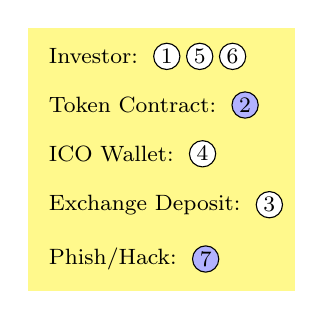
\begin{tikzpicture}[background rectangle/.style={fill=yellow!45}, show background rectangle]
\node (la) at(0, 0) {\footnotesize{Investor:}};
\node [below=5pt of la.south west, anchor=north west](lb) {\footnotesize{Token
Contract:}};
\node [below=5pt of lb.south west, anchor=north west](lc) {\footnotesize{ICO
Wallet:}};
\node [below=5pt of lc.south west, anchor=north west](ld)
{\footnotesize{Exchange Deposit:}};
\node [below=5pt of ld.south west, anchor=north west](le)
{\footnotesize{Phish/Hack:}};

\node [eoa, right=2pt of la.east, anchor=west] (ax) {\footnotesize{1}};
\node [eoa, right=2pt of ax.east, anchor=west] (bx) {\footnotesize{5}};
\node [eoa, right=2pt of bx.east, anchor=west] (cx) {\footnotesize{6}};


\node [ca, right=2pt of lb.east, anchor=west] (dx) {\footnotesize{2}};
\node [eoa, right=2pt of lc.east, anchor=west] (ex) {\footnotesize{4}};
\node [eoa, right=2pt of ld.east, anchor=west] (fx) {\footnotesize{3}};
\node [ca, right=2pt of le.east, anchor=west] (gx) {\footnotesize{7}};
\end{tikzpicture}

}


\begin{document}
\pgfplotstableread{
x a-min a-max a b-min b-max b
0 0.6000 0.9592 0.8022 0.5667 0.9596 0.8287
1 0.3871 0.9592 0.6761 0.5161 0.9694 0.7918
2 0.4706 0.9592 0.7186 0.6038 0.9645 0.8058
}\multilayertable

\pgfplotstableread{
x a-min a-max a b-min b-max b
0 0.6154 0.9583 0.8058 0.5667 0.9596 0.8287
1 0.5263 0.9388 0.7609 0.5161 0.9756 0.7918
2 0.6071 0.9485 0.7794 0.6038 0.9645 0.8058
}\timedensitytable

\pgfplotstableread{
x a-min a-max a b-min b-max b
0 0.546 1.0 0.848 0.615 0.958 0.806
1 0.158 0.951 0.496 0.526 0.939 0.761
2 0.245 0.907 0.593 0.607 0.949 0.779
}\symtable

\pgfplotstableread{
x a-min a-max a b-min b-max b
0 0.2381 0.6957 0.5660 0.546 1.0 0.848
1 0.1613 0.7429 0.3779 0.158 0.951 0.496
2 0.1923 0.6500 0.4358 0.245 0.907 0.593
}\multirelationtable

  \pgfplotsset{avg/.style={%
    legend style={
      legend columns=2,
      font=\footnotesize,
    },
    ybar,
    xtick pos = left,
    bar width=9pt,
    ymin=0,
    ymax=1.35,
    xmin=-0.5,
    xmax=2.5,
    scale only axis,
    xtick={0, 1, 2},
    ytick={0.2, 0.4, 0.6, 0.8, 1.0},
    xticklabels={\footnotesize{Precision}, Recall, $F_1$},
    xlabel=\empty,
    ylabel=\empty,
    width=0.2\textwidth,
    height=0.2\textwidth,
    every axis/.append style={font=\footnotesize},
legend image code/.code={%
                    \draw[#1, draw=none] (0cm,-0.1cm) rectangle (0.4cm,0.1cm);
                }
  }}

\title{I$^2$GL: An Identity Inference Approach for Blockchain based on Graph Deep Learning\\
%{\footnotesize \textsuperscript{*}Note: Sub-titles are not captured in Xplore and
%should not be used}
%\thanks{Identify applicable funding agency here. If none, delete this.}
}

%\author{\IEEEauthorblockN{Zaiyang Tang}\IEEEauthorblockN{Xiao Liu}
%\IEEEauthorblockA{\textit{Nebulas Research} \\
%\textit{Nebulas Research)}\\
%Beijing, China \\
%zaiyang.tang@nebulas.io}
%\and
%\IEEEauthorblockN{Xiao Liu}
%\IEEEauthorblockA{\textit{Peking University} \\
%\textit{name of organization (of Aff.)}\\
%Beijing, China \\
%lx\_lisa@pku.edu.cn}
%\and
%\IEEEauthorblockN{Peng Li}
%\IEEEauthorblockA{\textit{dept. name of organization (of Aff.)} \\
%\textit{name of organization (of Aff.)}\\
%City, Country \\
%email address}
%\and
%\IEEEauthorblockN{4\textsuperscript{th} Given Name Surname}
%\IEEEauthorblockA{\textit{dept. name of organization (of Aff.)} \\
%\textit{name of organization (of Aff.)}\\
%City, Country \\
%email address}
%\and
%\IEEEauthorblockN{5\textsuperscript{th} Given Name Surname}
%\IEEEauthorblockA{\textit{dept. name of organization (of Aff.)} \\
%\textit{name of organization (of Aff.)}\\
%City, Country \\
%email address}
%\and
%\IEEEauthorblockN{6\textsuperscript{th} Given Name Surname}
%\IEEEauthorblockA{\textit{dept. name of organization (of Aff.)} \\
%\textit{name of organization (of Aff.)}\\
%City, Country \\
%email address}
%}
\author{\IEEEauthorblockN{Xiao Liu\IEEEauthorrefmark{1}\IEEEauthorrefmark{2},
Zaiyang Tang\IEEEauthorrefmark{1}, Peng Li\IEEEauthorrefmark{3}, Xuepeng Fan\IEEEauthorrefmark{1},  Jinbo Zhang\IEEEauthorrefmark{2} and Song Guo\IEEEauthorrefmark{4}}
\IEEEauthorrefmark{1}Nebulas Research, China, Email: \{zaiyang.tang, xuepeng.fan\}@nebulas.io\\
\IEEEauthorrefmark{2}Peking University, China, Email: \{lx\_lisa, jinbozhang\}@pku.edu.cn\\
\IEEEauthorrefmark{3}The University of Aizu, Japan, Email: pengli@u-aizu.ac.jp\\
\IEEEauthorrefmark{4}Hong Kong Polytechnic University, Hong Kong, Email: song.guo@polyu.edu.hk\\
}


\maketitle

\begin{abstract}
Current cryptocurrencies, such as Bitcoin and Ethereum, enable anonymity by mapping user identity to public-keys only. On the other hand, deanonymization, i.e., inferring the real identity of blockchain users, is significant in many scenarios such as risk assessment and trade regulation. Existing work on blockchain deanonymization mainly focuses on Bitcoin that supports simple asset transferring. As the popularity of DApp platform blockchains with Turing-complete smart contracts, represented by Ethereum, blockchain deanonymization faces new challenges because of user diversity and complexity of activities. In this paper, we propose I$^2$GL, an identify inference approach based on graph deep learning to address these challenges. Specifically, I$^2$GL constructs a transaction graph and aims to infer the identity of nodes using graph embedding technique based on Graph Convolutional Networks. Furthermore, a series of enhancement has been proposed by exploiting unique features of blockchain transaction graph. The experimental results on Ethereum transaction records show that I$^2$GL significantly outperforms other state-of-the-art.
\end{abstract}

\begin{IEEEkeywords}
Cryptocurrency, Blockchain, Deanonymization, Graph deep learning
\end{IEEEkeywords}

% !TEX root = main.tex
\section{Introduction}
%\textcolor{red}{TBA.}
\textcolor{red}{
%Today cryptocurrencies have become a global phenomenon with the market capitalization of more than xxx billion dollars. 
%Blockchain technologies are gaining massive momentum in the last few years, largely due to the success of cryptocurrencies like Bitcoin and other altcoins. Blockchain is immutable ledger for recording transactions in append-only way, maintained within a distributed network. Pseudonymous is the born feature of blockchain, i.e., each account is associated with a public address, yet its actual identity is unknown. 
Blockchain technologies are gaining massive momentum in the last few years, largely due to the success of cryptocurrencies like Bitcoin and other altcoins. Anonymity in these cryptocurrencies is a very powerful feature. Within the system, users are identified by public-keys only. Transacting value across the blockchain can be done pseudonymously, and personal details can be veiled.
}

\textcolor{red}{
%Identity inferring, or deanonymization, plays an important role in blockchains. 
On the other hand, deanonymization attracts more and more people to think and concern as well. By tracking and inferring these accounts, people like traders, law-makers, financial security officers, etc, can have better understanding what is occurring on the blockchain. Thus, significant methods are proposed [XXX bitcoin deanonymizationpapers]. 
%There are many people, including traders, law-makers, financial security officers, etc, needs understand the behaviours on blockchains. 
}.

\textcolor{red}{
Challenges are accompanied by the rising of Ethereum, which is an open software platform based on blockchain technology that enables developers to build and deploy smart contracts.
%Ethereum denotes the practice of enabling users to build Turing-complete smart contract on blockchain. 
With such smart contracts, users could perform arbitrary behaviours, instead of simple token transfer. This brings two challenges for identify inferring. First, there are various identities and such identities are unforeseeable without expert knowledge and external information. Second, the behaviours performed by each identify are unpredictable.
}

\textcolor{red}{
%For example, ERC20 is one type of smart contracts. [introduce ERC 20 here].
%With the behaviours defined in ERC20 smart contracts, there are two new
%identities, investors and ICO wallets. More complicated, phishes and hackers
%disguise themselves as ERC20 accounts, which makes it even more difficult to
%identify phishes and hackers.
For example, there are more than $2500$ accounts are labeled as `Phish \& Hack' in Ethereum, which are fraud addresses related to phishing and hacks. Many of them are disguised as ICO (Initial Coin Offering) wallet or DApps (decentralized applications) such as casino, and it is hard to detect them without source code analysis. 
}

\textcolor{blue}{
It is not trivial to address these challenges. Existing methods [ref] highly
relies on experts to exhaustive enumerate all related features, which is easy
in well-defined currency blockchain systems, like Bitcoin. However, due to the arbitrary behaviours
defined in smart contracts, it is
almost impossible to enumerate corresponding related features in blockchains
like Etherum. %Some graph based methods [ref] are also facing the challenges from
%the unforeseeable identities and arbitrary behaviours.
}


\textcolor{blue}{
  We propose graph deep learning approach to address the challenges of deanonymization,
  unforeseeable identities and arbitrary behaviours.
}

%As the second major currency on the market with more than 10 billion dollars\footnote{At the time of this writing, the capitalization of Ethereum is about 11.8 billion dollars, once as high as more than 40 billion dolloars.} of capitalization, Ethereum is developed as a public, open-sourced blockchain-based platform~\cite{buterin2013ethereum}. Unlike Bitcoin, which was designed to be a currency, Ethereum aims to facilitate software processing using a token system called \emph{Ether} (ETH). Ethereum has the ability for users to build Turing-complete smart contract, which is a collection of code and data state that resides at a specific address on the Ethereum blockchain. Based on that, Ethereum can be applied to various scenarios beyond monetary exchange, such as voting, crowdfunding, lending, property rights protection and so on.

%From a logical perspective, the core elements in Ethereum include accounts and transactions. There are two types of accounts, namely \emph{Externally Owned Accounts} (EOAs) and \emph{Contract Accounts} (CAs). Both have an ETH balance and the major difference between is that EOAs are controlled by people who hold the public-private key pairs whereas CAs are ruled by executable codes inside. The transactions refer to the signed data package, recording messages to be sent from an account to another account on the blockchain. In Ethereum, various activities, such as money transfer, smart contract creation and invocation can be leveraged via transactions~\cite{chen2018infocom}.

%Ethereum is pseudonymous, i.e., each account is associated with a public address, but its actual identity is unknown. \textcolor{red}{On one hand, anonymity is in the reasons why people use cryptocurrency. Transacting value across the Ethereum network can be done pseudonymously, and personal details can be veiled. On the other hand, deanonymization attracts more and more people to think and concern as well. By tracking and inferring these accounts, we can have better understanding what is occurring on the blockchain. For instance, cryptocurrency team can make airdrop to the top valuable accounts~\cite{harrigan2018airdrops} and the fraud or cheating actions can be detected efficiently~\cite{monamo2016unsupervised}.}


%Although there exists some research efforts on deanonymization in Bitcoin, they are far from achieving identity inference in Ethereum. First, most deanonymization methods target on \textcolor{red}{rebuilding transaction flow on Bitcoin because the \emph{UTXO} (Unspent Transaction Output) model makes it hard to figure out the transaction trace~\cite{reid2013analysis,zhao2015graph,meiklejohn2013fistful}. However, there's really no such problems in Ethereum since Ethereum takes the \emph{Account/Balance} model and it is easy to reveal the transaction trace~\cite{buterin2013ethereum}.}

%\textcolor{red}{However, further deanonymization does not happen as expected in Ethereum. A proximate work is~\cite{chen2018infocom}, which has inferred the account identity by analyzing source codes (e.g., comments or keywords) of smart contracts. Such method relies on experts to exhaustive enumerate all related features, which is tedious, time-consuming and with low accuracy.}


%existing methods relies on experts to exhaustive enumerate all related features. The most relevant work to ours is~\cite{chen2018infocom}, which has inferred the account identity by analyzing source codes (e.g., comments or keywords) of smart contracts.}

%, but identify inference aims to reveal accounts' real identity, which is more challenging than traditional deanonymization.  This method is tedious, time-consuming and with low accuracy.}

%Second, existing methods gives only coarse-grained information, but identify inference aims to reveal accounts' real identity, which is more challenging than traditional deanonymization. The most relevant work to ours is~\cite{chen2018infocom}, which has inferred the account identity by analyzing source codes (e.g., comments or keywords) of smart contracts. This method is tedious, time-consuming and with low accuracy.

%On the one hand, most existing methods, however, are in the feature engineering manner, which relies on experts to exhaustive enumerate all related features~\cite{zhao2015graph,maesa2016analysis,chen2018infocom}. This way depends highly on the expertise. One can hardly expect the specialist familiar with all types of graphs, let alone ordinary users. Consequently, it's mechanical, rigid and time-consuming. On the other hand, previous methods exploit merely the node-level features and overlook the more important part, the relationship between nodes, namely the graph structural information. Due to the anonymity feature of Ethereum, little information is revealed in the node data, which results in the poor performance of these methods in blockchain data. Moreover, the inherent characteristic of blockchain data, that is the dynamic evolving, or more specifically, continuous growth in size, pose more challenges to the task. The work~\cite{chen2018infocom} analyze the Etherum from July, 2015 to June, 2017, which have only 48,261,952 transactions. Sadly, as the date of today, the transactions of the time period from Jan, 2018 to March, 2018 have exploded into 116,293,867, which can be hardly handled using traditional methods.~\footnote{The growth rate of Etherum transactions greatly slows down in 2018, so the period we selected could approximately represent the current maximum size of transactions in one quarter.}

%Chen et al.~\cite{chen2018infocom} conduct an investigation on Ethereum by leveraging graph analysis.

%\textcolor{red}{In this paper, we analyze Ethereum transactions and solve the identity inferring problem based on graph deep learning (graph DL)~\cite{battaglia2018relational}.}

\textcolor{red}{As a representative technique of Graph DL~\cite{battaglia2018relational}, }graph embedding provides an effective way to solve the graph analytics problem which convert the graph into a low dimensional space in which the graph information is preserve~\cite{cai2018comprehensive}. Based on the low dimensional vectors, some analytic tasks can be done effectively. Here we aim at determining the identity of accounts on other labeled accounts and the topology of the transaction graph. According to what we have learnt, this paper is the first work to analyze the transaction graph of cryptocurrency based on graph embedding techniques.

At the same time, we find that using such embedding techniques directly achieves poor effect on transaction graph. This is due to Ethereum transaction graph has many properties different from traditional networks, such as social media networks and citation graph. In Ethereum transaction graph, edges stand for different activities such as money transfer, contract creation and invocation, which can not be measured in a uniform weighted model. Besides, compared with other graphs, closeness features such as second-order proximity and asymmetric proximity in ETG are characteristic, which should be preserved. We also find that the relationship between a pair of nodes differs from another, even they have the same transaction frequency which could be expressed by time-density information.

Generally, our approach consists of three phases, \emph{graph construction}, \emph{graph embedding} and \emph{node classification}. In the construction phase, we construct the Ethereum transaction graph and divide it into multi-relation graphs to capture the different graph neighboring of transactions. In the embedding phase, we propose a XXX graph convolutional network and put the features of nodes and edges into representation. Last, a semi-supervised method is used for accounts classification.

In summary, this paper make the following major contributions.

(1) To the best of our knowledge, we are the first to analyze the transaction graph of cryptocurrency based on \textcolor{red}{graph DL} techniques. We propose a three-pronged approach to handle account inferring task and reveal the differences in analysis between Ethereum transaction graph and other traditional graphs.

\textcolor{red}{(2) To implement account inferring task, we propose a taxonomy of Ethereum accounts. The prominent identities are illustrated and provided for model training.}

%. Even the perfect categorization does not exist due to the blockchain anonymity and diversity in Ethereum. However, it is necessary to concern about the identities behind their on-chain transaction activities.
%we can still glean insight from examining the addresses with the most substantial balances by reviewing their on-chain transaction activity.

(3) To address these challenges, we introduce several techniques in data preprocessing and embedding. The evaluation through real data set shows the effectiveness of new approach.

\textcolor{red}{The rest of the paper is organized as follows. Section~\ref{sec:preliminary} introduces background knowledge of Ethereum and raises identity inferring problem. Section~\ref{sec:graph_analysis} gives an overview of our analysis procedure and illustrates the challenges. In Section~\ref{sec:model}, the detailed architecture is described. Section~\ref{sec:experiments} is experimental evaluation. Section~\ref{sec:relatedworks} presents the related works, and Section~\ref{sec:conclusion} concludes this paper.}




% !TEX root = main.tex

\section{Preliminary Analysis}
In the paper we analysis the Ethereum trading graph (ETG, for short) since Ethereum is the largest blockchain platform that supports cryptocurrency transferring and smart contracts. This section investigates the accounts and transactions on Ethereum since they are the basic unit of Ethereum and represent the nodes and edges in ETG respectively.


\subsection{Accounts}
In Ethereum, there are two kinds of accounts, external owned accounts and smart contracts, namely EOAs and SCs for short. The major difference between is that SCs are ruled by executable codes inside whereas EOAs are controlled by people who hold the public-private key pairs. Other than that, they do not look a whole lot different in Ethereum system. Both of them have unique addresses, the address of EOA is determined by the public key and the address of SC is encoded when SC is created. We use the terms address and account interchangeably in the remainder of this paper.

The real identities behind these addresses can be multitudinous and the anonymity of blockchain makes the identification more difficult. Generally, these addresses can be classified into different categories according to user roles on the blockchain.

%Here we take the category of address and the identity behind it as the same, although an individual or a group may has multiple address.

1) \emph{Miners \& Mining Pools}

Similar to Bitcoin, Ethereum takes \emph{Proof-of-Work} as its consensus protocol\footnote{Although Ethereum \emph{Casper} will abandon the PoW protocol, the current Ethereum is on the third stage \emph{Metropolis} which still mainly relies on solving hash problem.}. The \textbf{miners} are the individuals or groups who validate transaction information by solving the cryptographic puzzles. Whoever is the first to find a valid hash of block will get the reward in the form of ETH which is paid by users sending transactions.

In the early stage, most people take part in the mining process independently. With the more participants into this high profit industry, the mining competition gradually becomes fiercer. And an efficient solution is working together to solve the PoW problems. Miners with mining machines can register on a special institution named \textbf{mining pool} where aggregates all the registrants' computing power to solve mining problem and distributes the reward to the registrants according to their proportion of contributed computing power. As of September 2018, top $3$ mining pools takes more than 65\% of hash rate in Ethereum\footnote{Investoon, https://investoon.com/charts/mining/eth.}.
%The centralized institution is \textbf{mining pool} and these registrants are so called \textbf{cooperative miners}.


% And, more remarkable, the percentage of standalone miners declined and dropped to almost zero in the end of 2017. 

2) \emph{ERC-20 \& ICO}

ERC-20 is a technical standard used for smart contracts on the Ethereum blockchain for implementing tokens~\cite{erc-20-wiki}. It defines a common list of rules that an Ethereum token has to implement, giving developers the ability to program how new tokens will function within the Ethereum ecosystem. An ERC-20 token transfer happens in specific SCs which are called \textbf{ERC-20 token contracts}. %and the transferring process will be illustrated later. 

The ERC-20 token standard became popular with crowdfunding companies working on ICO cases due to the simplicity of deployment, together with its potential for interoperability with other Ethereum token standards~\cite{erc-20}. As of July 26 2018, there were more than 103,621 ERC-20 token contracts\footnote{Etherscan Token Tracker Page, https://etherscan.io/tokens}. Among the most successful ERC-20 token sales are EOS, Filecoin, Bancor, Qash, and Nebulas, raising over 60 million each\footnote{``Token Data, data and analytics for all ICO's and tokens", https://www.tokendata.io}.

Participants in the initial ICO round are \textbf{primary market investors} who buy the ERC-20 token from ERC-20 smart contracts of the crowdfunding companies. And these addresses where token sale proceeds are \textbf{ICO wallets}.

3) \emph{Exchanges}

The exchanges are the platforms for trading between ETH, fiat money (e.g., USD) and even other digital currency (e.g., BTC and ERC-20 tokens), which play an important role in Ethereum ecosystem. The exchanges can be categorized into centralized exchanges and decentralized exchanges (also known as DEXs) according to their architectures.

Most of the world’s cryptocurrency trading is done through centralized exchanges such as Binance, Huobi, OKEX etc\footnote{``Top 100 Cryptocurrency Exchanges by Trade Volume'', https://coinmarketcap.com/rankings/exchanges}. The centralized exchange allocates a deposit address to each user who wants to make transaction in the exchange. These addresses are called \textbf{exchange deposits} and belong to the exchange since users do not have the private key of these addresses. In recharge process, user transfers coins to the given deposit address from her own wallet and these coins will be transferred to the \textbf{exchange root} address automatically. In turn, users send requests to exchange to withdraw their coins from an address called \textbf{exchange withdrawal}. And in most cases, the exchange root and exchange withdrawal mean the same address.

%The exchange charges the user a commission for both recharge and withdraw services.

The DEXs are a new technology that facilitate cryptocurrency trading on a distributed ledger. Being completely on-chain, all orders interact with each other directly through the blockchain. This makes it fully decentralized, but also expensive and slow. Besides, another difference is that user will get a new address with corresponding private key when registers to the DEX, which means the address belongs to user itself instead of exchange. 
 
 %User calls the smart contract in the decentralized exchange address to start a transaction. Intuitively, the transaction will take a long time for making match and confirming compared with in centralized way.

%Since most ERC-20 token transactions happen via smart contracts and in a decentralized mechanism, some big exchanges which support both ETH and ERC-20 token transaction (e.g., Binance and Huobi) are mixture of centralized and decentralized exchange. 

4) \emph{Phishes \& Hacks}

Since virtual property transactions are now becoming increasingly commonplace and that leads to many security issues. At the same time, the frauds associated with ETH and ERC-20 tokens have also increased. We call these addresses related to frauds \textbf{phishes \& hacks}.

 In Ethersacan, there are more than $2500$ addresses are labeled as Phish/Hack, which takes up the highest proportion. Most of them are disguised as ERC-20 token sales or DApps such as casino. 

\begin{table}[htbp]
\caption{Typical Account Identities}
\begin{center}
\begin{tabular}{|p{1.8cm}|c|p{3.9cm}|}
\hline
\textbf{Identity} & \textbf{Type}& \textbf{Description} \\
\hline
Miner & EOA & The node who take part in the block validation process. \\ \hline
Mining Pool & EOA & The pooling of resources by miners, who share their processing power over a network.\\ \hline
ERC-20 Token Contract & SC & Smart contract that allow customers to transfer ERC-20 tokens. \\ \hline
Primary Market Investor & EOA & Participants in the initial ICO round. \\ \hline
ERC-20 Token Sale & EOA\&SC & Address that allows customers to buy ERC-20 tokens. \\ \hline
Exchange Deposit & EOA\&SC & Address for user to deposit ETH at exchange. \\ \hline
Exchange Root \& Withdrawal & EOA\&SC & Address collects ETH from deposit addresses and withdraw ETH to users. \\ \hline
Phish \& Hack & EOA\&SC & Fraud address related to phishing and hacks. \\ \hline
%\multicolumn{4}{l}{$^{\mathrm{a}}$Sample of a Table footnote.}
\end{tabular}
\label{tab1}
\end{center}
\end{table}



%Phishing is the name given to the latest online scam where millions of unwary Americans are getting their identities stolen.

%We've seen increased use of sophisticated forms and letterhead to send what appears to be legitimate World Bank Group correspondence, as well as several schemes that reference the Bank.


\subsection{Transactions}
Transaction is the basic unit in each block which represents an action between two accounts. Transaction can be categorized as external one and internal one based on the sponsor of the transaction. A transaction is the external one if it is sent from an EOA while the internal one results from executing a smart contract due to an external transaction~\cite{chen2018infocom}. Note that an external transaction may lead to many internal transactions.

Four types of transaction can be found by parsing Ethereum blocks, including \emph{CALL}, \emph{CRATE}, \emph{REWARD} and \emph{SUICIDE}. As shown in Fig.?, ETH transferring and smart contract invoking comes with a \emph{CALL} transaction usually and \emph{CREATE} is used to deploy smart contracts. \emph{REWARD} transactions appears on the head of block, which depicts the reward that block miner obtained from system. The sender of \emph{REWARD} transaction is a special address \emph{0x00...00}. In the \emph{SUICIDE} transaction, the smart contract will execute destroy method to kill itself at the end of it's cycle. \emph{CALL}, \emph{CREATE} and \emph{SUICIDE} transactions can be either external transactions or internal transactions since the initiator can be both EOA and SC.

Various activities are realized on Ethereum based on the above mentioned transactions. Money transfer, contract creation and contract invocation are three major activities happening on Ethereum\cite{chen2018infocom}. \textcolor{gray}{The on-chain assets include ETH coin and ERC-20 token.} An typical ETH transfer is shown in Fig. ? in where the initiate address and target address can be both EOA and SC. In the \emph{CALL} transaction information, the amount to be transferred is a non-zero number. However, the process of ERC-20 token transfer is more complicated. The sponsor A (also called initiator) make a \emph{CALL} transaction to the ERC-20 smart contract to tell that he want to transfer ERC-20 token to somebody B. Then the smart contract will check the request and complete the deal if A has enough ERC-20 token. Note that the target address of the \emph{CALL} transaction is the ERC-20 SC instead of B address and the transfer value is $0$ ETH since the actual transfer happens in the smart contract where the ERC-20 token is transferred from A account to B account in the smart contract inner database. 



\section{AIGL Approach}
\label{sec:approach}
In this section, we propose AIGL, a cryptocurrency anonymity identification approach based on graph deep learning. We first give an overview of AIGL, and then present technical details including graph construction, embedding and node classification.

%we are the first to analyze cryptocurrency transactions and solve the identity inferring problem based on graph deep learning.

\subsection{Overview}
\label{subsec:methodology}
%In AIGL, identity inferring task is turned into node classification problem, simply, predicting the identity of accounts on a small sample of labeled accounts and the topology of the transaction graph.
\textcolor{red}{The basic idea of AIGL is to present the accounts in cryptocurrency and associated transactions as a graph. In the graph, accounts are represented as nodes with low dimensional vectors by embedding technique. Then, the identify inference is to classify nodes on the graph by given a labeled training set.}

Specifically, AIGL consists of three phases: graph construction, graph embedding and node classification as shown in Fig.~\ref{fig:architecture}.

\begin{figure}[htbp]
	\centering
	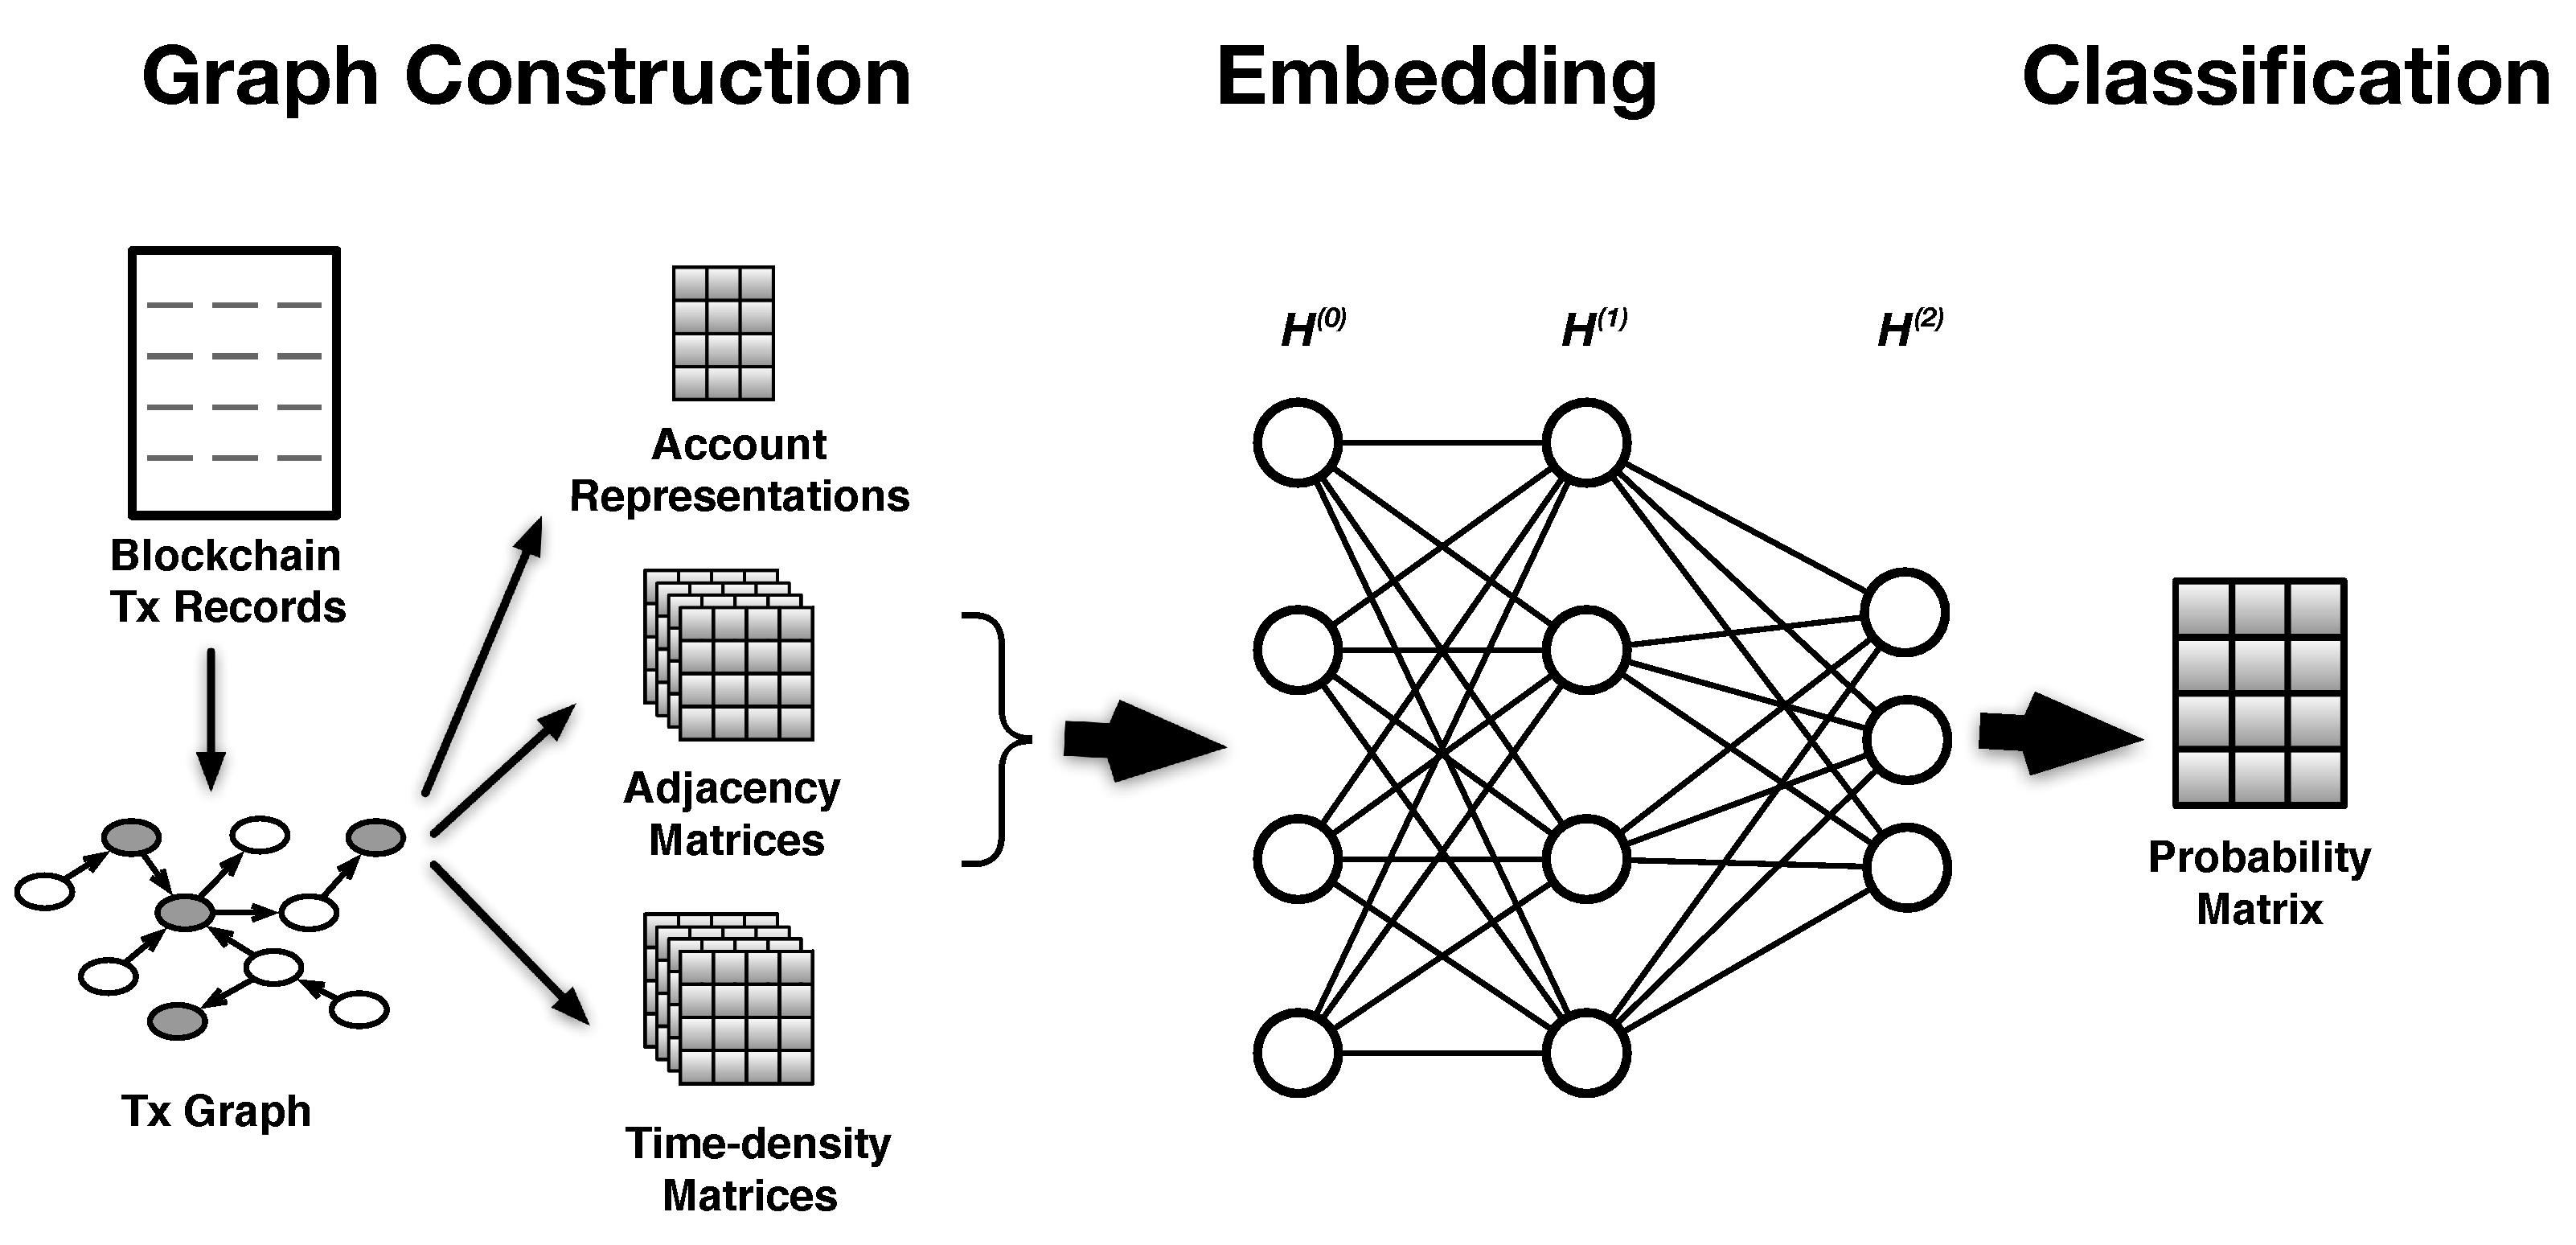
\includegraphics[width=3.5in]{fig/architecture.eps}
	\caption{Overall architecture.}
	\label{fig:architecture}
\end{figure}

\textbf{Phase 1: Graph construction}. We construct the blockchain transaction graph as a directed graph $G_{t}=(V,E)$, where node $v \in V$ represents an account that can be an EOA or CA. We use the terms account and node interchangeably in the remainder of this paper. The total number of accounts is depicted as $|V|=N$.

$E$ contains ordered pairs, i.e., $E=\{(v_i,v_j)|v_i,v_j \in V\}$, where $(v_{i},v_{j})$ indicates the direction of transaction (e.g., assets transfer or smart contract invocation) from $v_i$ to $v_j$. \textcolor{red}{Within $E$, each edge has weight, and the specific method for calculating is detailed in the following sub-section.}

%Analogously, the number of edges in ETG is represented as $|E|$.

\textbf{Phase 2: Graph embedding}.
\textcolor{red}{Graph embedding provides an effective yet efficient way to solve the graph analytics problem~\cite{cai2018comprehensive}.} The embedding process can be defined as follows: given $G_{t}=(V,E)$, we represent each node $v$ in a low-dimensional vector space $\vec{y_v}$. Based on such vectors, node classification can then be computed efficiently with high accuracy.

Typical network embedding techniques, such as random-walk based and deep learning based models, use the pure network structure to map into the embedding space~\cite{goyal2018capturing}. Our model is primarily motivated as an extension of GCNs (Graph Convolutional Networks)~\cite{kipf2016semi,schlichtkrull2018modeling}, which puts the features of nodes and edges into the representation, since it shows effectiveness for entity classification in large-scale relational data.


\textbf{Phase 3: Node classification}.
The final objective of AIGL is to predict account identities on transaction graph. Given a labeled accounts set, supervised or semi-supervised methods can be used for entities classification. A intuitive way is simply stacking GCN layers of the form with a softmax ($\cdot$) activation on the output of the last layer~\cite{schlichtkrull2018modeling}. \textcolor{blue}{A cross-function can be the minimizing objective for training.}

\textcolor{red}{Last but not the least, the categorization is important to performance of classification. For cryptocurrencies that do support smart contract, such as Ethereum, we propose a coarse taxonomy which is illustrated in TABLE~\ref{table:identity}.} 

 %To be frank, the perfect categorization does not exist because Ethereum and Ethereum-like blockchains are still in a development stage. \textcolor{red}{For accounts in Ethereum, we propose} a coarse but effective taxonomy.

\subsection{Graph Construction}
The transaction graph can be constructed based on original transaction records synchronized from the blockchain. In AIGL, the graph is represented as several matrices: (a) \emph{account representations}, (b) \emph{adjacency matrices}, and (c) \emph{time density matrices}.


%(1) a node representation matrix that captures the structural and additional information of accounts, (2) a list of adjacency matrices which describe different relations, and (3) a list of time-density matrices that represent transaction intensiveness between each pair of nodes.

%Different from other studies~\cite{kipf2016semi,schlichtkrull2018modeling}, the graph is translated into 

\paragraph{Account representations} To encode the overall structural and additional information of accounts, we denote the account representations as a feature matrix $X \in \mathbb{R}^{N \times d}$, where each account contains the following $d$ pre-defined features.

\begin{itemize}
	\item \emph{in-degree}: the number of incoming edges of a node, that is, the number of transactions initiated by an account.
	\item \emph{out-degree}: the number of outgoing edges of a node, that is, the number of transactions which point to an account.
	\item \emph{weighted in-degree}: the value summation of incoming edges of a node, which represents the total crptocurrencies received by an account.
	\item \emph{weighted out-degree}: the value summation of edges outgoing to a node, which represents the total cryptocurrencies sent from an account.
	%\item eccentricity
	%\item clustering coefficient
	\item \emph{account type}: whether the account is a smart contract or normal one.
\end{itemize}

\paragraph{Adjacent matrices} Different from other networks, edges in transaction graph stand for heterogeneous activities such as money transfer, contract creation and contract invocation. Obviously, such %multi-relations can not be measured in a uniform weighted model.
activitities should be represented as different edge types instead of being measured in uniform weighted graph.

To address the challenge, we divide the raw transaction graph into several sub-graphs and capture the relations of graph neighboring nodes using adjacent matrices. The set of adjacency matrices, $\{A^1,A^2,\dots,A^R|A^i\in \mathbb{R}^{N \times N}\}$, describes the $R$ relations among $N$ nodes in transaction graph. It is conceivable that, the strategy of division has a large influence on classification performance.

In AIGL, four major transactions are considered, including (1) \texttt{CALL} with value, (2) \texttt{CALL} without value, (3) \texttt{CREATION} and (4) \texttt{REWARD}, which represent the relations of cryptocurrency transferring, smart contract invocation, smart contract deployment and mining rewarding, respectively. \textcolor{red}{More specifically, transaction is regarded as type 1 that an account transfer some ETH (cryptocurrency in Ethereum) to another one. And the ERC-20 token transferring is regarded as type 2 since it is a contract invocation without any ETH.}

On one hand, for relations of \textcolor{red}{type 2, type 3 and type 4}, we calculate the frequency of repeated edges between a pair of nodes as the adjacent weight in the corresponding relation adjacent matrix. For cryptocurrency transferring, on the other hand, it is not sensible to use the assets amount directly as the adjacent weight. That is because the accounts have varied enormously in terms of cryptocurrency transferring which will lead to underflow and overflow in the process of training.

 Taking Ethereum transaction as an example, the amount of assets transferring is discretized into three ranges: (1) small transfers which the transaction value is less than 1 ETH (the cryptocurrency used in Ethereum); (2) medium transfers which the transaction value is between 1 ETH and 10 ETH and (3) major transfers which the transaction value is above 10 ETH. Then the ETH transferring matrix can be calculated in a similar way with other relations.

%forward transactions introduced above and 4 reverse relations in order to pass information from the opposite direction. Besides, a self loop as a special relation type is included to retain information of the previous layer in the GCN network.

%Specially, the adjacent matrices are modified to preserve the asymmetric proximity of transaction graph, which will be addressed in detail later.

\paragraph{Time-density matrices}
\textcolor{red}{As noted above, the value $a^r_{ij}$ in adjacent matrix $A^r$ is equal to accumulated frequency of edges between $v_i$ and $v_j$ in relation $r$. }

%Even in a single relation graph, there may be multiple edges between the same node pairs. This occurs quite naturally since an account may transfer or invoke to another account repeatedly for a period of time, which is quite different from the knowledge graphs and citation networks.

%Intuitively, a simple solution is to merge those edges by frequency or weight summation \textcolor{red}{in the same way as what is doing in adjacency matrices. 
\textcolor{red}{In fact, more information could be exploited on transaction graph. Within each block, transactions are labeled with block height which can be regarded as timestamp. These repeated edges are located at different time intervals along the time axis. Based on such information, we expand on these adjacent features to open a new dimension.}


 
\begin{figure}[htbp]
\centering
\begin{tabular}{c}
	\subfigure[Time variance histogram of whole nodes.]{
		\label{fig:high_order}
		%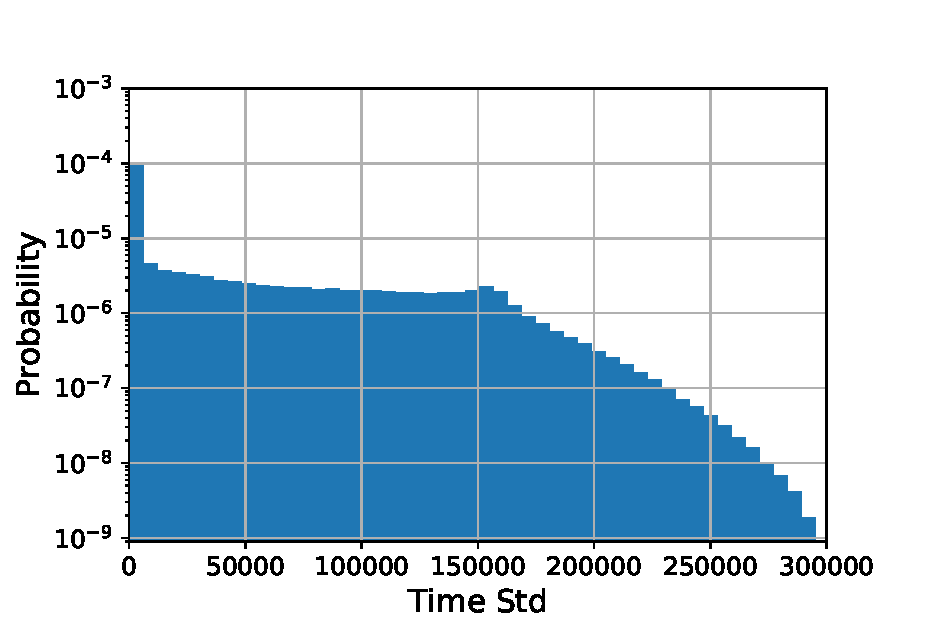
\includegraphics[width=0.22\textwidth]{fig/all_time_std_pdf.eps}
    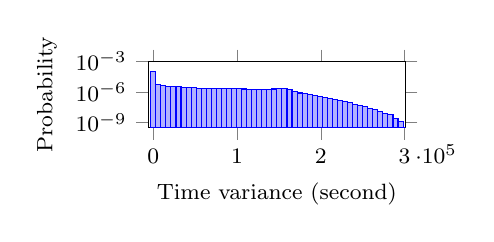
\begin{tikzpicture}
\begin{axis}[ymax=0.001,ybar,ymode=log,bar width=6023.807139652907,log origin=infty,xmin=-6023.807139652907,ytick align=outside,enlargelimits=0,
width=.40\textwidth,
height=.20\textwidth,
ylabel=Probability,
xlabel=Time variance (second),
every x tick scale label/.style={at={(xticklabel cs:1)},anchor=south west},
  label style={font=\footnotesize},
tick label style={font=\footnotesize} ,
]
\addplot  plot coordinates {
(0.0, 9.451382865223466e-05)
(6023.807139652907, 5.4237855234498505e-06)
(12047.614279305813, 4.160561994558263e-06)
(18071.421418958722, 3.567714777734051e-06)
(24095.228558611627, 3.385128656276782e-06)
(30119.03569826453, 3.165308635083816e-06)
(36142.842837917444, 2.9615307529739165e-06)
(42166.64997757035, 2.6626153921894407e-06)
(48190.45711722325, 2.5490152149843527e-06)
(54214.26425687616, 2.3890921746281617e-06)
(60238.07139652906, 2.275444535473124e-06)
(66261.87853618198, 2.248248838151831e-06)
(72285.68567583489, 2.156718467673447e-06)
(78309.49281548779, 2.138350693042835e-06)
(84333.2999551407, 2.0591366985764506e-06)
(90357.1070947936, 2.0862137410228693e-06)
(96380.9142344465, 2.0135969575995206e-06)
(102404.72137409942, 2.000948347937872e-06)
(108428.52851375232, 1.9544830989369192e-06)
(114452.33565340523, 1.9188391745245435e-06)
(120476.14279305813, 1.8834088288869425e-06)
(126499.94993271104, 1.8642104701322076e-06)
(132523.75707236395, 1.8633324240581345e-06)
(138547.56421201685, 1.8347365992133192e-06)
(144571.37135166978, 1.9392715439779758e-06)
(150595.17849132267, 2.1352419353211166e-06)
(156618.98563097557, 2.1487685910568386e-06)
(162642.79277062847, 1.6649889352174985e-06)
(168666.5999102814, 1.0367825656806102e-06)
(174690.4070499343, 7.939434987619423e-07)
(180714.2141895872, 6.496829018892185e-07)
(186738.02132924012, 5.151757357311993e-07)
(192761.828468893, 4.3131047016972446e-07)
(198785.6356085459, 3.5105231280444205e-07)
(204809.44274819884, 2.852225882239295e-07)
(210833.24988785174, 2.272003544101756e-07)
(216857.05702750463, 1.7961974958539996e-07)
(222880.86416715756, 1.4827113164349042e-07)
(228904.67130681046, 1.1445449230418602e-07)
(234928.47844646336, 8.545524088479658e-08)
(240952.28558611625, 6.371766780774196e-08)
(246976.09272576918, 4.777045262457526e-08)
(252999.89986542208, 3.780344313509607e-08)
(259023.70700507498, 2.6009148572545693e-08)
(265047.5141447279, 1.8557622430411254e-08)
(271071.3212843808, 1.31232291611476e-08)
(277095.1284240337, 8.305841241232658e-09)
(283118.9355636866, 5.624241069063257e-09)
(289142.74270333955, 2.7053311471443514e-09)
(295166.54984299245, 1.3526655735721757e-09)
(301190.35698264535, 3.0850267467435584e-10)
};\end{axis}
\end{tikzpicture}

	%\caption{Example of a high-order proximity caption.}
	}\\
	\subfigure[Time variance histogram of hack\&phish nodes.]{
		\label{fig:asymmetric}
		%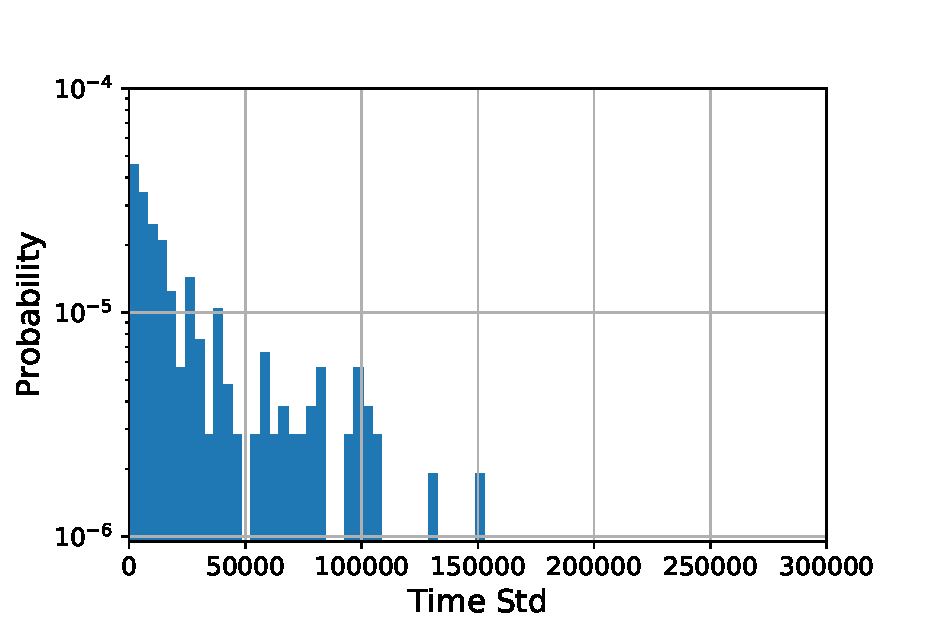
\includegraphics[width=0.22\textwidth]{fig/fake_time_std_pdf.eps}
    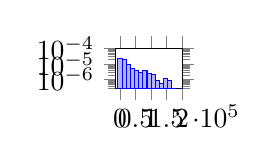
\begin{tikzpicture}
\begin{axis}[ymax=0.0001,ybar,ymode=log,bar width=13410.783587930588,log origin=infty,xmin=-13410.783587930588,ytick align=outside,enlargelimits=0,
width=.20\textwidth,
every x tick scale label/.style={at={(xticklabel cs:1)},anchor=south west},
]
\addplot  plot coordinates {
(0.0, 2.1630081044550223e-05)
(13410.783587930588, 1.9637836737815332e-05)
(26821.567175861175, 8.822796215540222e-06)
(40232.350763791765, 5.122913931604e-06)
(53643.13435172235, 3.699882283936222e-06)
(67053.91793965294, 2.8460632953355556e-06)
(80464.70152758353, 3.984488613469778e-06)
(93875.48511551411, 2.561456965802e-06)
(107286.2687034447, 2.2768506362684445e-06)
(120697.0522913753, 8.538189886006666e-07)
(134107.83587930587, 5.692126590671111e-07)
(147518.61946723645, 1.1384253181342222e-06)
(160929.40305516706, 8.538189886006666e-07)
(174340.18664309764, 2.8460632953355556e-07)
(187750.97023102822, 0.0)
(201161.75381895882, 2.8460632953355556e-07)
};\end{axis}
\end{tikzpicture}

	}
\end{tabular}
\caption{Time variance histogram of accounts in Ethereum.}
\label{fig:time_std}
\end{figure}

Fig.~\ref{fig:time_std} illustrates the distribution of time variance when transaction happens of whole accounts and hack \& phish accounts in Ethereum. We observe that the time variance distribution of hack \& phish accounts is more concentrated compared with other accounts, since they are more active in a short period. This insight inspires us to use time information such as the variance of time transaction happens.

To describe time-density information, we use a set of matrices $\{T^1,T^2,\dots,T^R|T^i\in \mathbb{R}^{N \times N}\}$. Given a sequence $\{h_{ij1}^r,h_{ij2}^r,\dots,h_{ijm}^r | h_{ijk}^r>0\}$ as the block height of $m$ transactions in relation $r$ between node $v_i$ and $v_j$, the time-density of each relation $r$ is computed as%Equation \ref{eq:time}

\begin{equation}
t{ij}^r=g(\sqrt{Var[\frac{1}{m}\sum_{k=1}^m h_{ijk}^r]})
\label{eq:time}
\end{equation}

\noindent where $g(\cdot)$ is the function of squash which can be logarithmic function.

\subsection{Embedding}
\label{sec:rGCN layers}
Based on the above input matrices, we propose a multi-layer Graph Convolutional Network with the following layer-wise propagation rule:

%The method can be understood as a more abstract propagation rule:
\begin{equation}
H^{(l+1)}=\delta(\sum_{r\in R} (K^r\odot (D^r)^{-1}A^r)H^{(l)}W_r^{(l)}),\forall r
\end{equation}
\noindent where $H^{(l)}$ is the matrix of activations of the $l$-th layer, and here the $0$ layer is set as the account representations, that is, $H^{(0)}=X$. We use $\delta(\cdot)$ to denote an activation function such as the ReLU$(\cdot)$ = max$(0,\cdot)$. $A^r$ is the adjacent matrix of relation $r$, and $D^r$ is a diagonal matrix of relation $r$ where $d^r_{ii}=\sum_{j}a^r_{ij}$. $\odot$ indicates point-wise multiplication.

The edge weight $a^r_{ij}$ in adjacency matrix $A^r$ is defined as \emph{first-order proximity} which represents similarity between nodes $v_i$ and $v_j$~\cite{tang2015line}. Further, \emph{second-order proximity} compares the neighborhood of two nodes and treat them as similar if they have a similar neighborhood~\cite{goyal2018graph}.

In cryptocurrency transaction graph, it turns out that second-order proximity plays important role in preserving the local structure as well as first-order proximity. As shown in Figure \ref{fig:high_order}, nodes $a$ and $c$ are smart contracts and node $b$ is normal user. Obviously, $a$ is not adjacent to $c$  but they have similar neighbor structure. Embedding models with first-order proximity will keep them far apart although they have similar connection structures, while embedding with second-order proximity captures this similarity.

 We feed the input into a GCN model with 2 hidden layers, as a trade-off between preserving second-order proximity and introducing noise. 
 
 The input of the $l$-th layer is $H^{(l)}=\{h_1^{(l)},h_2^{(l)},...,h_N^{(l)}|h_i^{(l)}\in \mathbb{R}^{N \times d^{(l)}}\}$. Hence the method can be understood as special cases of the forward updating process.

\begin{equation}
h_i^{(l+1)}=\delta(\sum_{r\in R} \sum_{j \in N_i^r} \frac{\tau_{ij}^r}{\hat c_{i,r}}W_r^{(l)}h_j^{(l)})
\end{equation}

\noindent where $h_i^{(l)}$ is the hidden state of node $v_i$ in the $l$-th layer of the neural network. $r \in R$ represents a kind of relation, $N_i^r$ denotes the set of neighbor indices of node $v_i$ under relation $r$, and $k_{ij}^r$ is the time-density of transactions from node $v_i$ to $v_j$ which is represented in Eq.~(\ref{eq:time}).



\begin{figure}[htbp]
	\centering
	\subfigure[Second-order proximity]{
		\label{fig:high_order}
    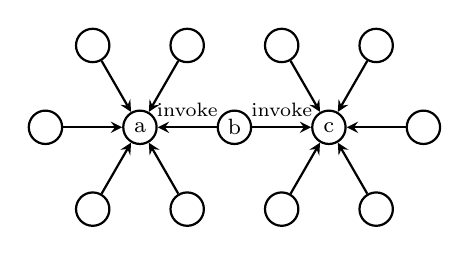
\begin{tikzpicture}
\tikzset{
  base/.style={draw, on grid, align=center, minimum height=2.8ex},
  pn/.style={base, circle},
}


\tikzmath{\r=1.2;}

\node [pn, thick] (a) at (0, 0) {};
\node at (a) {\footnotesize a};
\node [pn, thick] (b) at (\r, 0) {};
\node at (b) {\footnotesize b};
\node [pn, thick] (c) at (2*\r, 0) {};
\node at (c) {\footnotesize c};

\node[pn, thick] (a1) at ({\r*cos(60)}, {\r*sin(60)}) {};
\node[pn, thick] (a2) at ({\r*cos(120)}, {\r*sin(120)}) {};
\node[pn, thick] (a3) at ({\r*cos(180)}, {\r*sin(180)}) {};
\node[pn, thick] (a4) at ({\r*cos(240)}, {\r*sin(240)}) {};
\node[pn, thick] (a5) at ({\r*cos(300)}, {\r*sin(300)}) {};

\node[pn, thick] (b1) at ({2*\r + \r*cos(60)}, {\r*sin(60)}) {};
\node[pn, thick] (b2) at ({2*\r + \r*cos(120)}, {\r*sin(120)}) {};
\node[pn, thick] (b3) at ({2*\r + \r*cos(0)}, {\r*sin(0)}) {};
\node[pn, thick] (b4) at ({2*\r + \r*cos(240)}, {\r*sin(240)}) {};
\node[pn, thick] (b5) at ({2*\r + \r*cos(300)}, {\r*sin(300)}) {};

\draw[->, >=stealth, thick] (a1)-- (a);
\draw[->, >=stealth, thick] (a2) -- (a);
\draw[->, >=stealth, thick] (a3) -- (a);
\draw[->, >=stealth, thick] (a4) -- (a);
\draw[->, >=stealth, thick] (a5) -- (a);

\draw[->, >=stealth, thick] (b1) -- (c);
\draw[->, >=stealth, thick] (b2) -- (c);
\draw[->, >=stealth, thick] (b3) -- (c);
\draw[->, >=stealth, thick] (b4) -- (c);
\draw[->, >=stealth, thick] (b5) -- (c);

\draw[->, >=stealth, thick] (b) -- (a) node [midway, above] {\scriptsize invoke};
\draw[->, >=stealth, thick] (b) -- (c) node [midway, above] {\scriptsize invoke};
\end{tikzpicture}

		%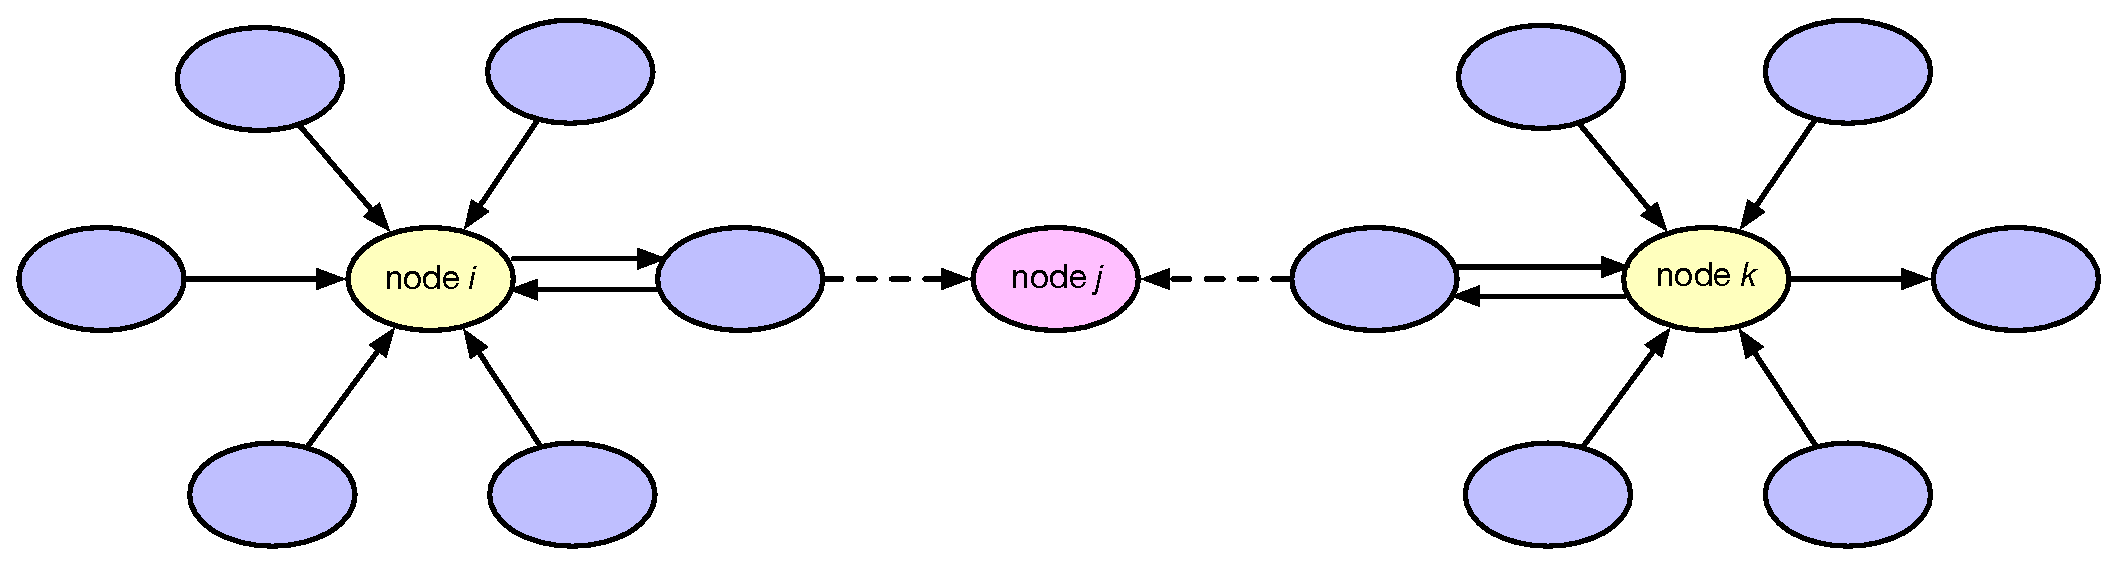
\includegraphics[width=2.0in]{fig/high_order_proximity.eps}
	%\caption{Example of a high-order proximity caption.}
	}
	\subfigure[Asymmetric proximity]{
		\label{fig:asymmetric}
    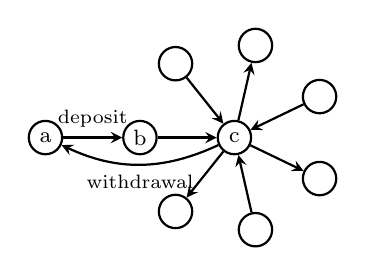
\begin{tikzpicture}
\tikzset{
  base/.style={draw, on grid, align=center, minimum height=2.8ex},
  pn/.style={base, circle},
}


\tikzmath{\r=1.2;}

\node [pn, thick] (a) at (0, 0) {};
\node at (a) {\footnotesize a};
\node [pn, thick] (b) at (\r, 0) {};
\node at (b) {\footnotesize b};
\node [pn, thick] (c) at (2*\r, 0) {};
\node at (c) {\footnotesize c};

%\node[pn] (a1) at ({\r*cos(60)}, {\r*sin(60)}) {};
%\node[pn] (a2) at ({\r*cos(120)}, {\r*sin(120)}) {};
%\node[pn] (a3) at ({\r*cos(180)}, {\r*sin(180)}) {};
%\node[pn] (a4) at ({\r*cos(240)}, {\r*sin(240)}) {};
%\node[pn] (a5) at ({\r*cos(300)}, {\r*sin(300)}) {};

\node[pn, thick] (b1) at ({2*\r + \r*cos(360.0/14)}, {\r*sin(360.0/14)}) {};
\node[pn, thick] (b2) at ({2*\r + \r*cos(360.0*3/14)}, {\r*sin(360.0*3/14)}) {};
\node[pn, thick] (b3) at ({2*\r + \r*cos(360.0*5/14)}, {\r*sin(360.0*5/14)}) {};
\node[pn, thick] (b4) at ({2*\r + \r*cos(360.0*9/14)}, {\r*sin(360.0*9/14)}) {};
\node[pn, thick] (b5) at ({2*\r + \r*cos(360.0*11/14)}, {\r*sin(360.0*11/14)}) {};
\node[pn, thick] (b6) at ({2*\r + \r*cos(360.0*13/14)}, {\r*sin(360.0*13/14)}) {};

%\draw[->, >=stealth] (a1)-- (a);
%\draw[->, >=stealth] (a2) -- (a);
%\draw[->, >=stealth] (a3) -- (a);
%\draw[->, >=stealth] (a4) -- (a);
%\draw[->, >=stealth] (a5) -- (a);

\draw[->, >=stealth, thick] (b1) -- (c);
\draw[->, >=stealth, thick] (c) -- (b2);
\draw[->, >=stealth, thick] (b3) -- (c);
\draw[->, >=stealth, thick] (c) -- (b4);
\draw[->, >=stealth, thick] (b5) -- (c);
\draw[->, >=stealth, thick] (c) -- (b6);

\draw[->, >=stealth, thick] (a) -- (b) node [midway, above] {\scriptsize deposit};
\draw[->, >=stealth, thick] (b) -- (c) node  {};
\draw[->, >=stealth, thick] (c) to [out=205, in=335]  node [midway, below] {\scriptsize
withdrawal}  (a);
\end{tikzpicture}

		%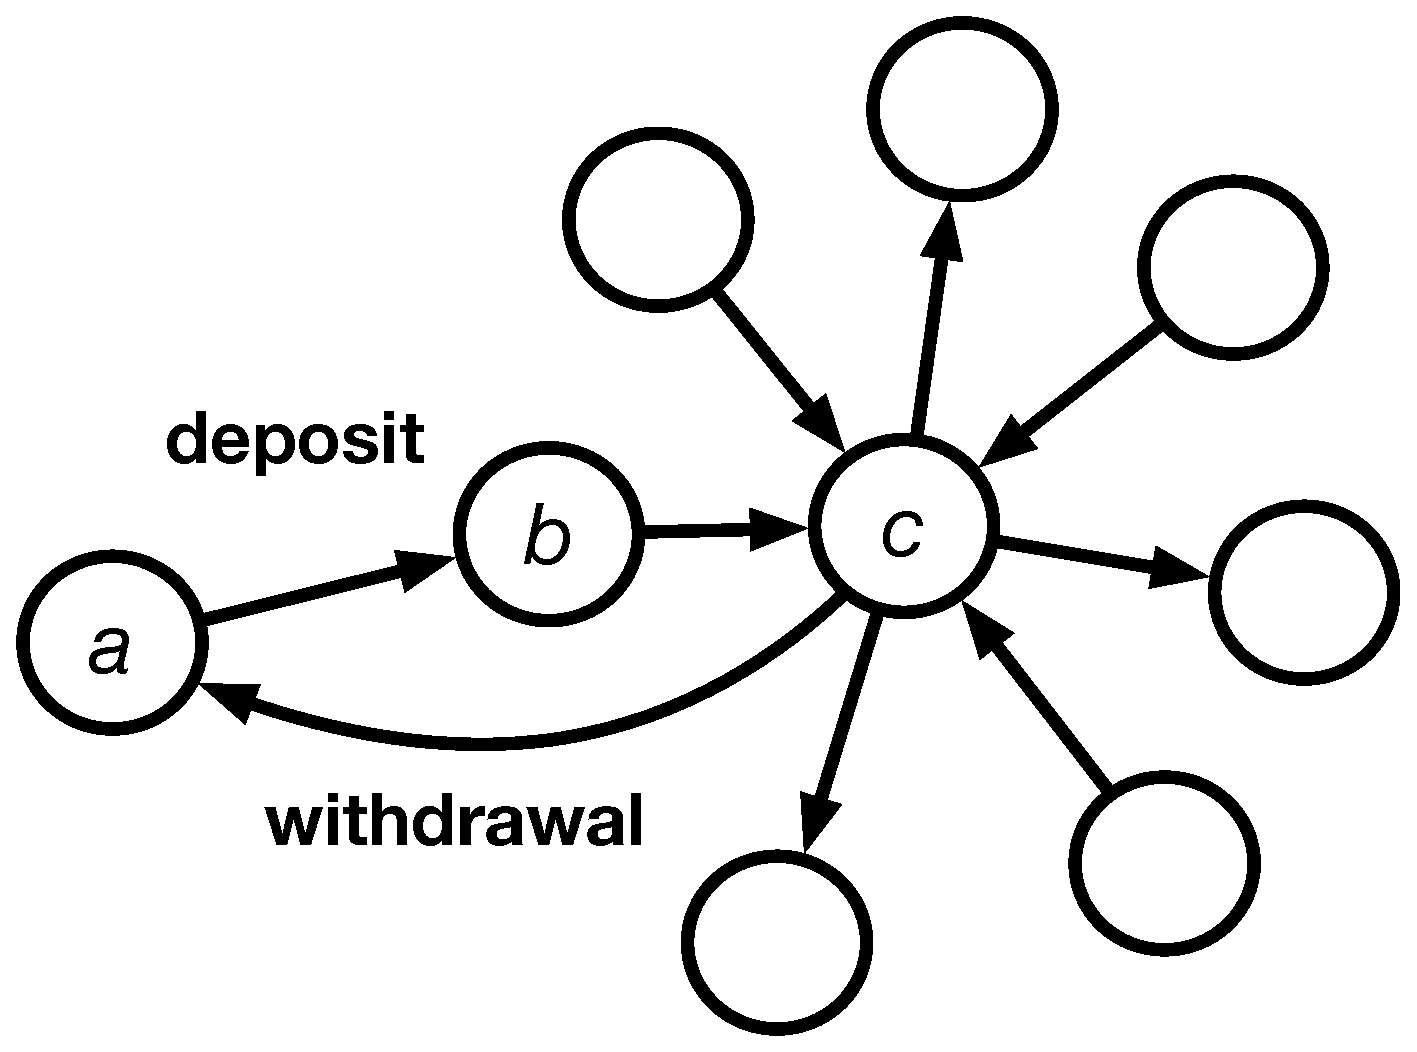
\includegraphics[width=1.5in]{fig/asymmetric.eps}
	}
	\caption{Examples of second-order and asymmetric proximity.}

\end{figure}


Another overlooked closeness, \emph{asymmetric proximity} should also be preserved in transaction graph. For instance, as shown in Figure. \ref{fig:asymmetric}, node $a$ denotes cryptocurrency trader and node $b$ and $c$ are cryptocurrency exchange accounts. Consequently, edge $(a,b)$ stands for deposit process while edge $(c,a)$ is withdrawal process. Generally, edge weight can be $A_{ab}=A_{bc}=A_{ca}$ since deposit and withdrawal come in pairs in symmetric model. However, the proximity $(a,c)$ is not equal to proximity $(c,a)$ due to their asymmetric local structures.

Unlike the asymmetric proximity preserving approach based on random walk~\cite{zhou2017scalable}, our method is based on a kind of non-probability graph embedding model.
 %Zhou et. proposed a scalable asymmetric proximity preserving graph embedding method based on random walk~\cite{zhou2017scalable}. In their model, the probability that $v_a$ arrives at $v_c$ is far less than the one that $v_c$ arrives at $v_a$, as the out degree of $v_c$ is bigger than the out degree of $v_a$
 
To preserve the asymmetric proximity, the coefficient $\hat c_{i,r}$ is introduced as:
\begin{equation}
\hat c_{i,r}=\frac{1}{d_i^r\cdot |N_i^r|}
\end{equation}

\noindent where $d_i^r=\sum_{j}A^r_{ij}$, and $|N_i^r|$ is used for normalization.



\subsection{Node Classification}
The output of the last layer indicates the probability that each node being assigned to each class.

The output of the last \textcolor{red}{GCN} layer is regarded as a probability matrix $P=\{p_1,p_2,...,p_N|p_i\in \mathbb{R}^{N \times m}\}$, where $p_i=\{p_{i,1},p_{i,2},...,p_{i,m}\}$ describes the probability of classifying node $v_i$ into $m$ categories.

We utilize the cross-entropy loss function as the training objective:
\begin{equation}
L=-\sum_{i=1}^T\sum_{j=1}^m y_{i,j}\log p_{i,j}+\lambda ||\theta||^2
\end{equation}

\noindent where $T$ is the number of training samples, $y_{i,j}$ is the true probability of node $v_i$ belonging to category $j$. $\theta$ is the set of all parameters and $\lambda$ is the coefficient for $L_2$  regularization.

%% !TEX root = main.tex

\section{Ethereum Trading Graph Analysis}
Based on effective graph analytics, we can investigate more information hidden behind transaction data on blockchain. For example, by analyzing the Ethereum trading graph (ETG, for short), accounts can be classified as different identities. 

In this section, we illustrate the construction of ETG and analyze some features which makes it different from other networks or graphs.


 %we first introduce the definition of the basic concepts in trading graph embedding, and then construct multi-layer trading graph.

\subsection{Problem Definition and Modeling}
Generally, we consider the ETG as a directed graph $G=(V,E)$, where node $v \in V$ represents an account and $e \in E$ depicts the edge between two nodes. Actually, $V$ is the set of all addresses in Ethereum includes both EOAs and SCs and we use the terms address, account and node interchangeably in the remainder of this paper. $E$ is a set of ordered pairs, where $E=\{(v_i,v_j)|v_i,v_j \in V\}$. The order of an edge indicates the direction of activity (e.g., assets transfer and smart contract invocation) from $v_i$ to $v_j$.
%In our definition, each edge associates with a weight $w$, which will be discussed later. Hence, $G$ is a weighted directed graph.

The problem can be defined as follows: given ETG $G=(V,E)$, we aim to represent each node $v$ in a low-dimensional vector space $\vec{y_v}$. By representing ETG as a set of low dimensional vectors, graph analysis algorithms can then be computed efficiently. 

Typical network embedding techniques such as random-walk based and deep learning based models use the pure network structure to map into the embedding space~\cite{goyal2018capturing}. Our model is primarily motivated as an extension of GCNs (Graph Convolutional Networks) since it shows effectiveness for entity classification in large-scale relational data~\cite{kipf2016semi}. Generally, a multi-layer Graph Convolutional Network with the following layer-wise propagation rule:

\begin{equation}
H^{(l+1)}=\delta(\tilde{D}^{-\frac{1}{2}}\tilde{A}\tilde{D}^{-\frac{1}{2}}H^{(l)}W^{(l)})
\label{eq1}
\end{equation}

where $H^{(l)}$ is the matrix of activations in the $l$-th layer, and $W^{(l)}$ is a trainable weight matrix in the $l$-th layer. $\delta(\cdot)$ denotes an activation function such as the ReLU$(\cdot)$ = max$(0,\cdot)$. $\tilde{A}=A+I_N$ where $A$ is the adjacency matrix of the graph $G$ and $I_N$ is the identity matrix. $\tilde{D}$ is a diagonal matrix which $\tilde{D}_{ii}=\sum_{j}\tilde{A}_{ij}$.

 The method can be understood as special cases of a simple differentiable message-passing framework.

\begin{equation}
h_i^{(l+1)}=\delta(\sum_{j \in N} \frac{1}{c_{i,j}}W^{(l)}h_j^{(l)})
\label{eq:gcn}
\end{equation}

where $h_i^{(l)}$ is the hidden state of node $v_i$ in the $l$-th layer of the neural network. And $c_{ij}$ is a problem-specific normalization constant which can defined in advance such as $c_{i,j}=\sqrt{d_i d_j}$ where $d_i$ is the degree of node $v_i$.

The approach outperforms other methods such as deepwalk~\cite{perozzi2014deepwalk} in experiments on citation networks and knowledge graph dataset. However, we found that using such GCN model directly achieves poor effect on ETG which has many different properties from traditional networks (such as social media networks and citation graph). It brings the following challenges.

\begin{itemize}
\item In the original ETG, there are different relations such as assets transfer and smart contract invocation. Those relations are radically different from one another and can not be measured in a uniform weighted graph.
\item Even taking a single relation graph, there are multiple edges between two nodes. For instance, repeated transactions between the same account pairs often happen. A simple method is to merge them and it will lose some information.
\item Asymmetric
%In ETG, two nodes are more similar if they have similar connection structures instead of they are just connected by an edge with larger weight simply or have similar neighborhoods. Using node adjacency as the input, most graph embedding techniques can not preserve such higher order proximity.
\end{itemize}

\subsection{Multi-relations}

\begin{figure}[htbp]
	\centering
	\label{fig_graph_split}
	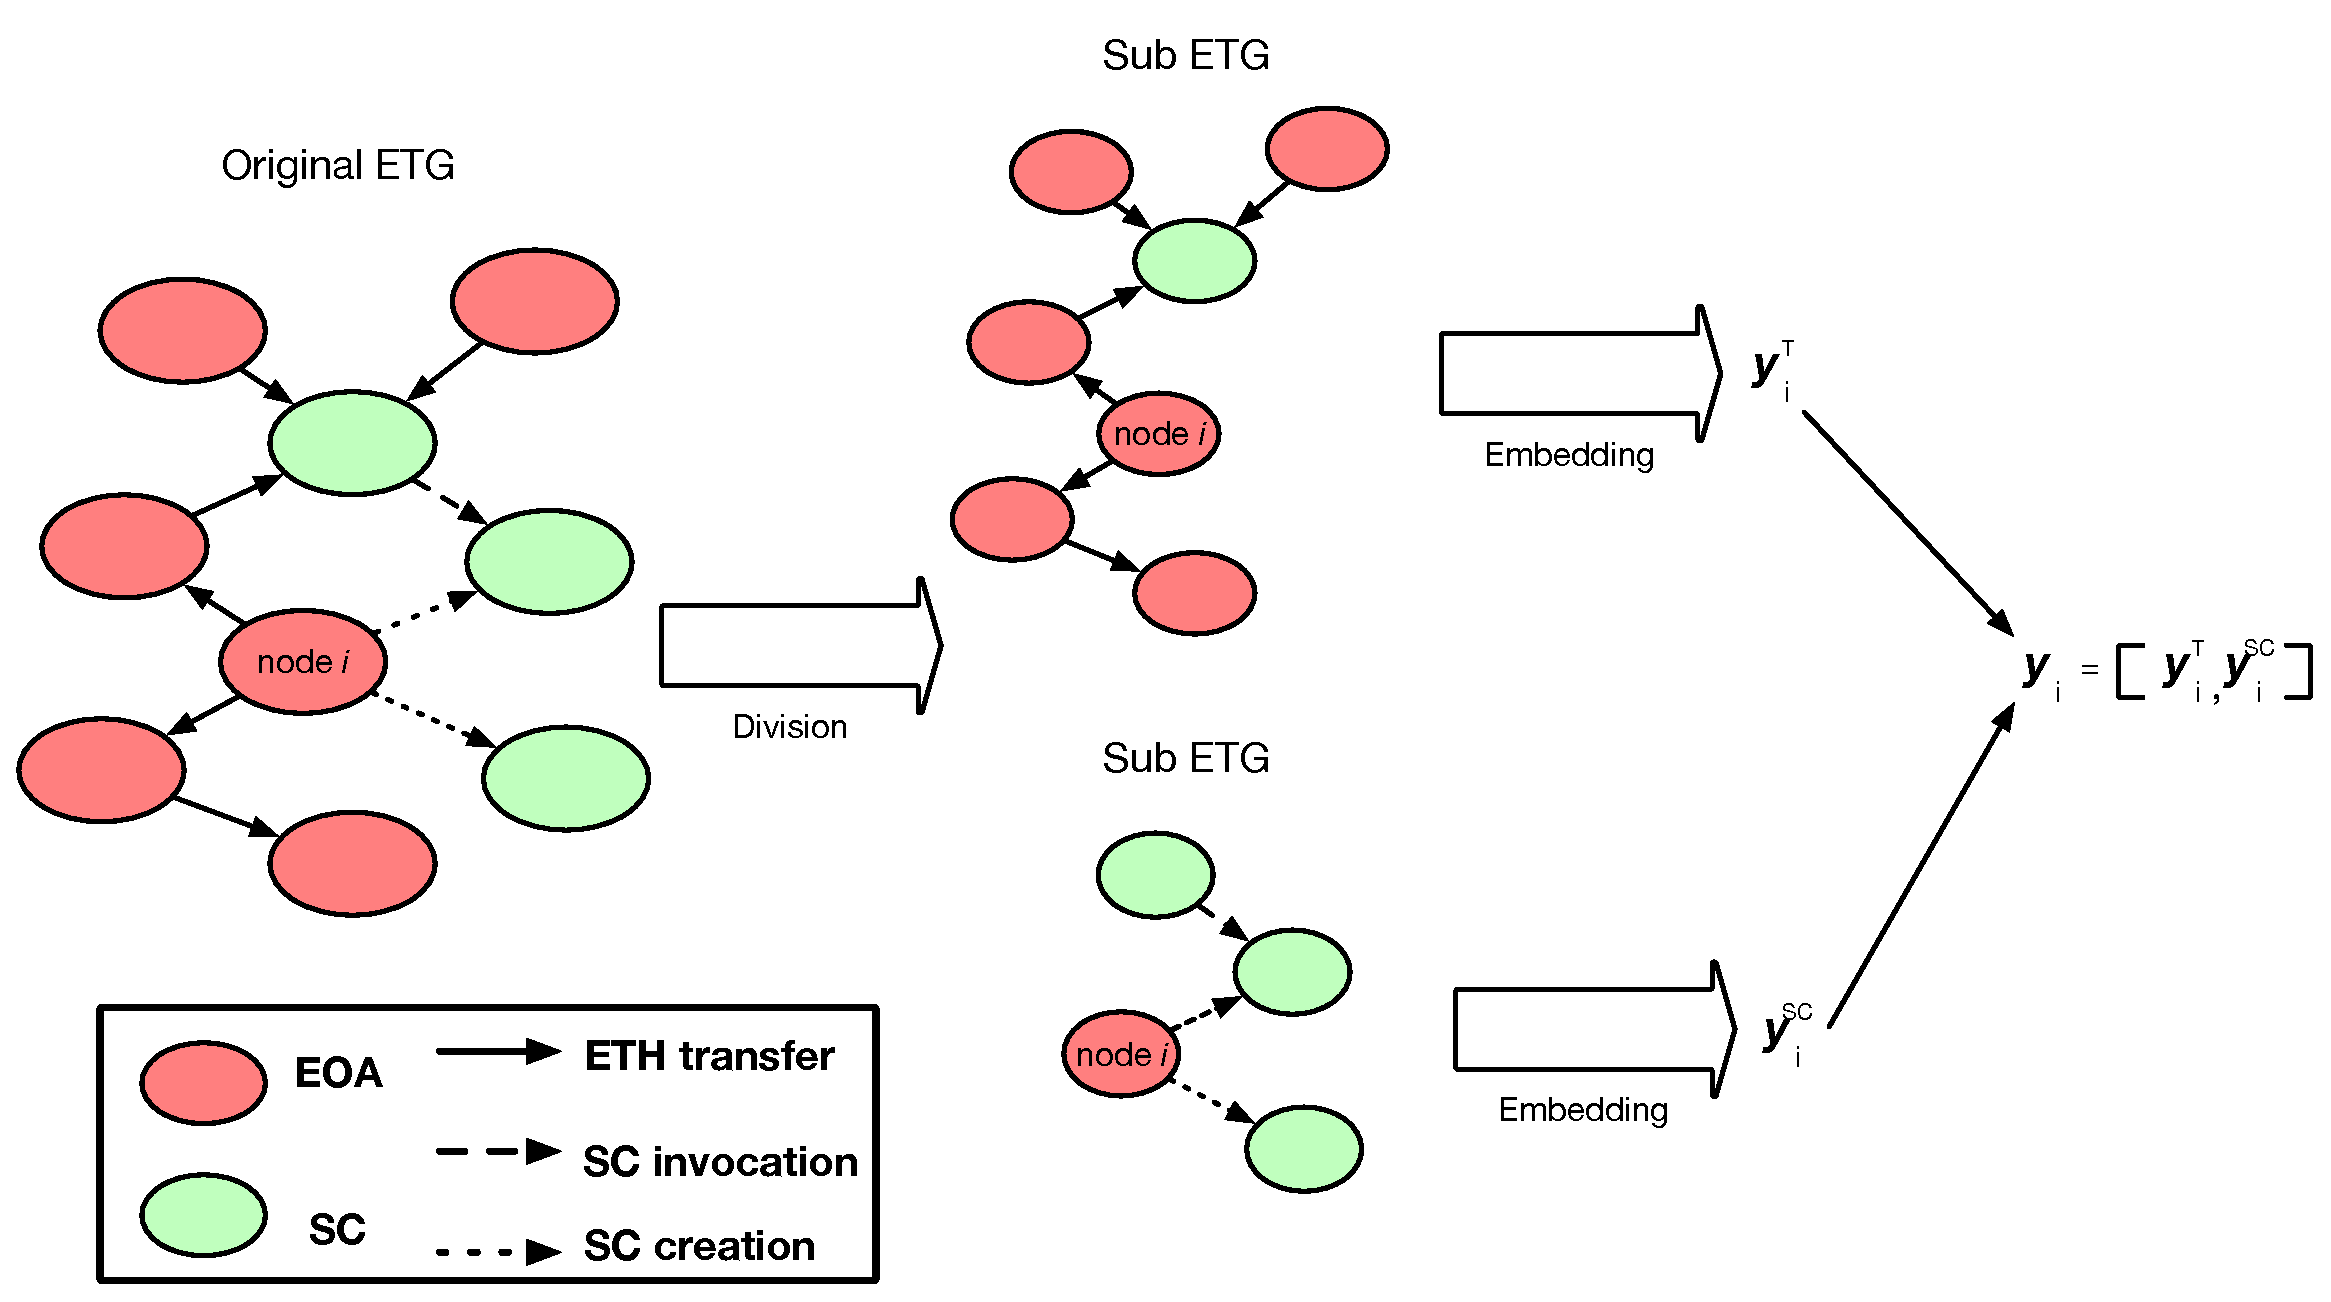
\includegraphics[width=3.5in]{fig/graph_split.eps}
	\caption{Example of a figure caption.}


	%\caption{Example of a figure caption.}
	%\label{fig_graph_split}
\end{figure}

In ETG, edges stand for different activities such as money transfer, contract creation and contract invocation, which can not be measured in a uniform weight model. For example, a weight of assets transfer maybe the ETH amount, however an invocation to smart contract does not have such numerical value. This inspired us to divide the raw ETG into different relation graphs.

%\textbf{Definition 1.} $G^{T}=\{V^T,E^T\}$, where $V^T$ is the subset of $V$. $E^T=\{(v_i,v_j,w)|v_i,v_j \in V^T,w \in \mathbb{R^+}\}$ where an edge $(v_i,v_j)$ indicates that there is at least one ETH transfer from node $v_i$ to $v_j$. And $w$ is the summation of all transferred ETH amount from $v_i$ to $v_j$ for a period of time.

%Actually, $G^T$ represents the ETH trading activities in Ethereum, and each node in $V^T$ has at least one ETH transaction.

%\textbf{Definition 2.} $G^{SC}=\{V^{SC},E^{SC}\}$, where $V^{SC}$ is the subset of $V$. $E^{SC}=\{(v_i,v_j,w)|v_i,v_j \in V^{SC},w \in \mathbb{R^+}\}$ where an edge $(v_i,v_j)$ indicates that there is at least one smart contract creation or invocation from node $v_i$ to $v_j$. And $w$ is the summation of \emph{CREATE} transaction and \emph{CALL} with $0$ ETH transactions for a period of time. 


%And $w$ is the summation of all transferred ETH amount from $v_i$ to $v_j$ for a period of time.

Relational Graph Convolutional Networks (rGCNs) is proposed to develop an encoder model for edges in the relational graph~\cite{schlichtkrull2018modeling}. The propagation model can be expressed as

\begin{equation}
h_i^{(l+1)}=\delta(\sum_{r\in R} \sum_{j \in N_i^r} \frac{1}{c_{i,r}}W_r^{(l)}h_j^{(l)}+W_0^{(l)}h_i^{(l)})
\label{eq:rgcn}
\end{equation}

where $r \in R$ represents a kind of relation and $N_i^r$ denotes the set of neighbor indices of node $v_i$ under relation $r$. Besides, single self-connection is introduced as a special relation type to each node. %compared with Eq.\ref{eq:gcn}

In return, we divide the edge set into four relations, CALLs with ETH, CALLs without ETH, CREATIONs and REWARDs, according to the their transaction type. Note that the ERC-20 token transfers are categorized as CALLs without ETH which includes normal smart contract invocations as well. The reason is that ERC-20 token transfer is a kind of contract invocation and the transaction value is $0$ in an ERC-20 \emph{CALL} transaction. Another reason is that even converting some ERC-20 tokens into ETH is available, the exchange-rate fluctuations make the unification meaningless.


\subsection{Time-density}
\label{section:time}
Even in a specific relation graph, there are repeated edges between the same node pairs. This occurs quite naturally since an account may transfer or invoke to another account repeatedly.

Note that these activities are located at different time intervals along the time axis which are characterized by the block height. Intuitively, a simple solution is to merge those edges by weight summation and it will lose time information. 

Here we introduce an index named time-density which can be represented as strictly increasing function of block height variance.

\begin{equation}
\tau_{ij}^r=g(var(\texttt{bn}_{ij}^r))
\label{eq:time}
\end{equation}

where $\texttt{bn}_{ij}^{r}$ is the block height set of relation $r$ between node $v_i$ and $v_j$. And the new adjacency matrix in relation $r$ can be represented as 

\begin{equation}
\hat{A}=\tilde{D}^{-\frac{1}{2}}\tilde{A}\tilde{D}^{-\frac{1}{2}}V
\label{eq:?}
\end{equation}

where $V_{ij}=\tau_{ij}$.

\textcolor{red}{TBA}

\subsection{High Order and Asymmetric Proximity}
In weighted graph, the edge weight $A_{ij}$ in adjacency matrix $A$ is generally treated as a measure of similarity between nodes $v_i$ and $v_j$. And the higher the edge weight, the more similar the two nodes are expected to be. Edges weight $A_{ij}$ is called \emph{first-order proximity} between nodes $v_i$ and $v_j$. 

Further, \emph{second-order} compares the neighborhood of two nodes and treat them as similar if they have a similar neighborhood~\cite{goyal2018graph}. Two nodes in ETG are more similar if they have similar connectivity structures instead of they are just connected by an edge with larger weight or share similar neighborhoods. As shown in Figure \ref{fig:high_order}, nodes $v_a$ and $v_c$ are smart contracts and node $v_b$ is normal user. Obviously, $v_a$ is not adjacent to $v_c$  but they have similar neighbor structure. Embedding models with \emph{first-order proximity} and \emph{second-order proximity} will keep them far apart although they have similar connection structures. 

\begin{figure}[htbp]
	\centering
	\subfigure[Example of a high-order proximity caption.]{
		\label{fig:high_order}
		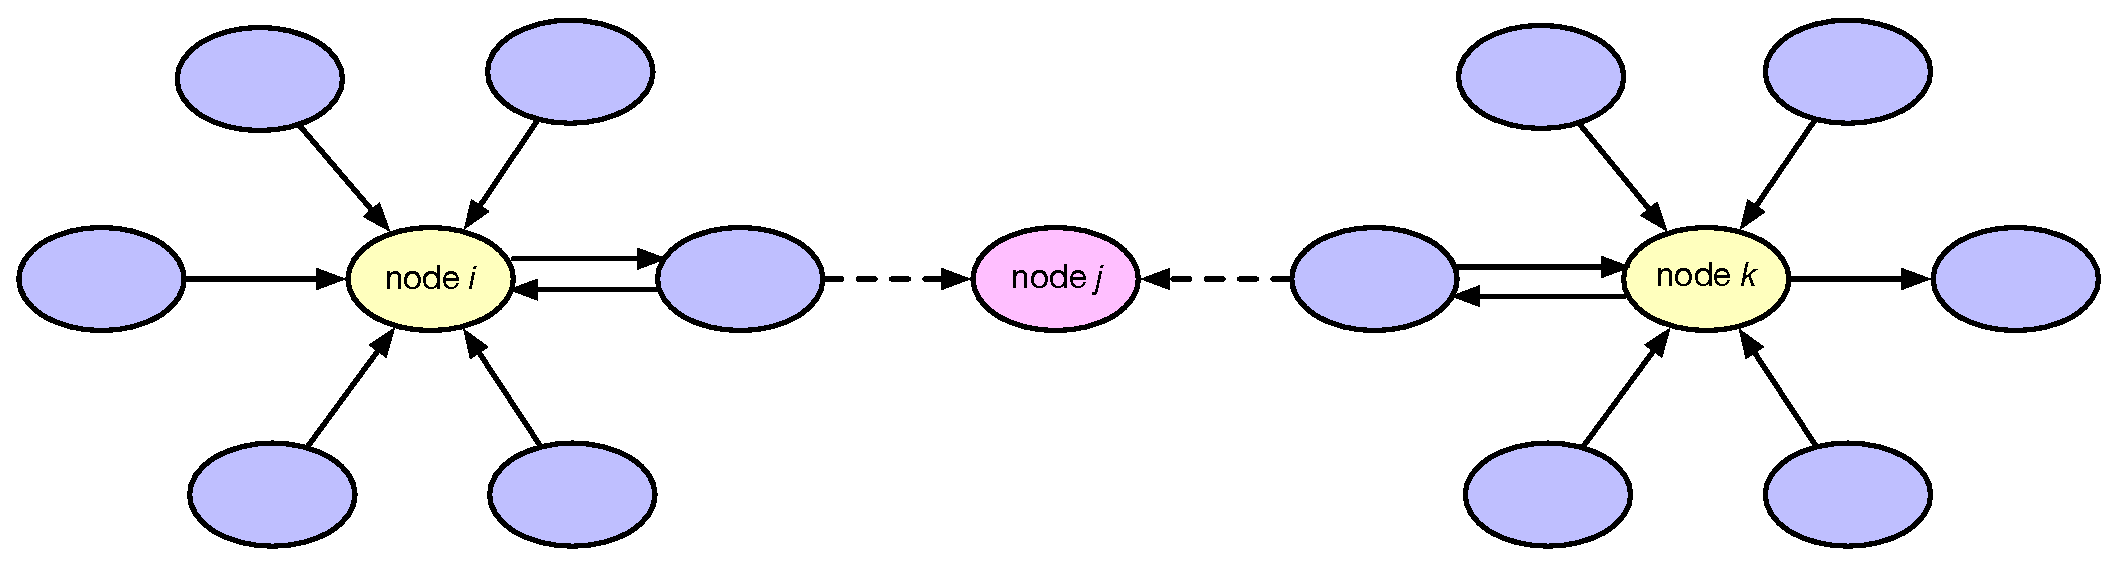
\includegraphics[width=2.0in]{fig/high_order_proximity.eps}
	%\caption{Example of a high-order proximity caption.}
	}
	\subfigure[Example of an asymmetric proximity caption.]{
		\label{fig:asymmetric}
		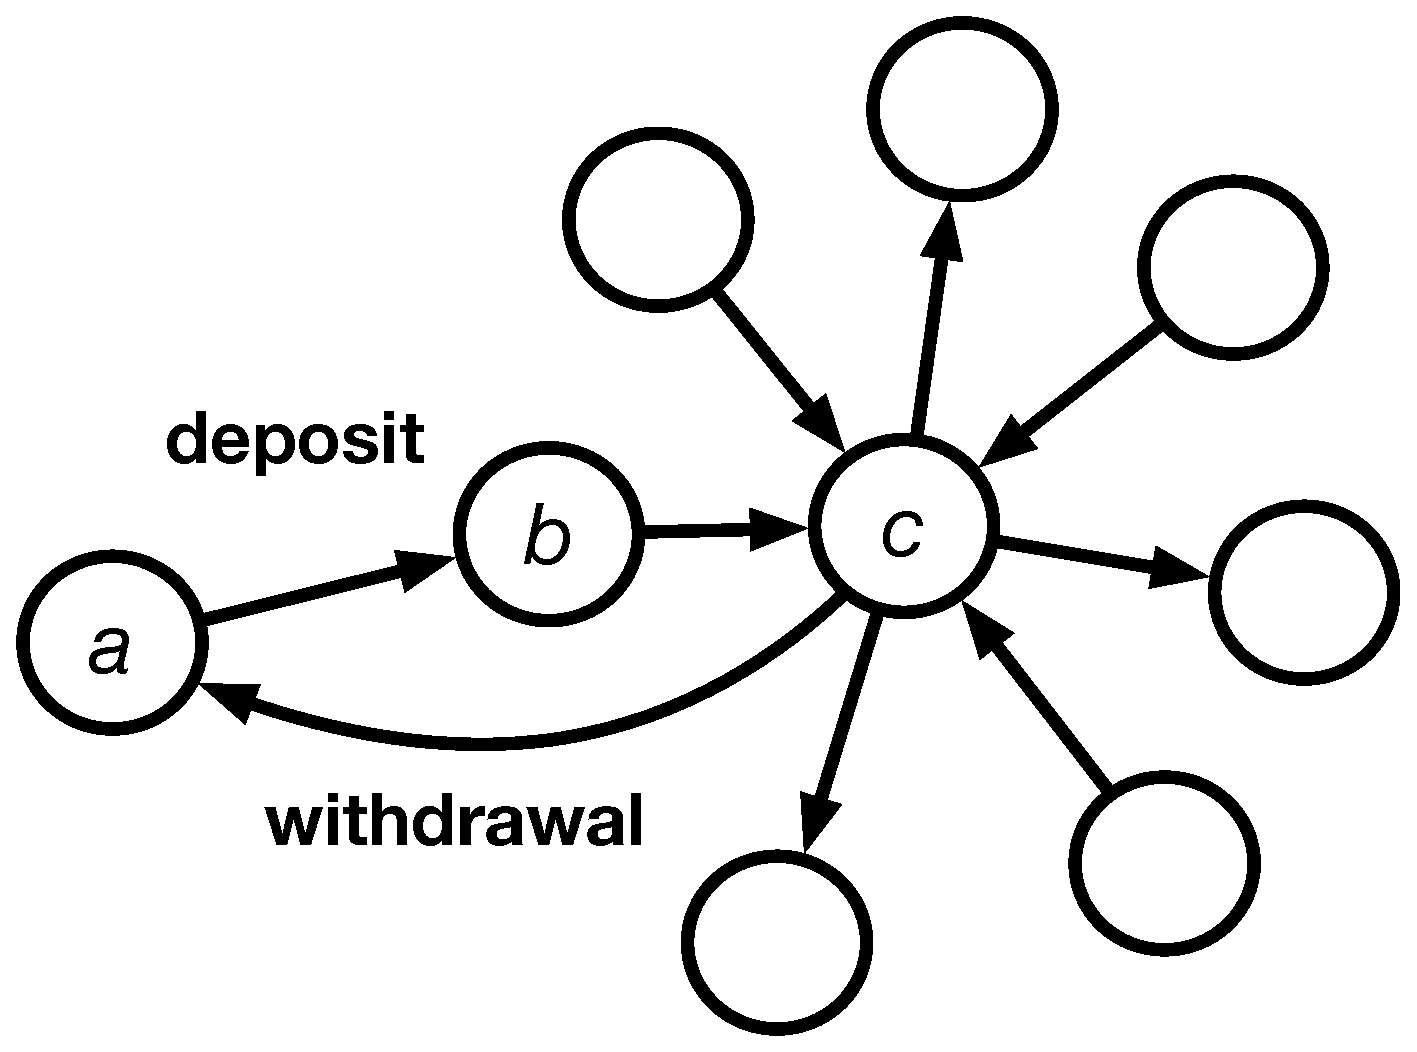
\includegraphics[width=1.5in]{fig/asymmetric.eps}
	}
	\caption{Examples of an asymmetric proximity.}

\end{figure}

To preserve higher order proximities, the hidden layer number in our model is set as 2.

\textcolor{red}{TBA}

Another property of closeness in ETG is \emph{asymmetric proximity}. For instance, as shown in Figure. \ref{fig:asymmetric}, node $v_a$ is a Ethereum investor address and node $v_c$ is an exchange root address. Generally, edge weight can be $A_{ab}=A_{bc}=A_{ca}$ since deposit and withdrawal come in pairs in symmetric model. However, the proximity $(v_a,v_c)$is not equal with proximity $(v_c,v_a)$ due to their asymmetric local structures.


 Zhou et. proposed a scalable asymmetric proximity preserving graph embedding method based on random walk~\cite{zhou2017scalable}. In their model, the probability that $v_a$ arrives at $v_c$ is far less than the one that $v_c$ arrives at $v_a$, due to their asymmetric local structures. However, there is no research on asymmetric proximity in GCN model.
 
 To preserve asymmetric proximity, we..
 
 \textcolor{red}{TBA.}


%% !TEX root = main.tex

\section{System Model}
Figure. x depicts the overall architecture of our ETG node classification model. The input consists of three parts (Section \ref{sec:input}): a node feature matrix that captures the structural information of nodes, a list of time-density matrices that represent transaction intensiveness between each pair of nodes, and a list of adjacency matrices which describe different relations. We feed the input into two rGCN layers (Section \ref{sec:rGCN layers}), as a trade-off between preserving high-order proximities and introducing noise. The output of the last layer indicates the probability that each point being assigned to each class.

\subsection{Input}
\label{sec:input}
\textbf{Node representations.} We use a feature matrix $X \in \mathbb{R}^{N \times d}$ to encode the overall structural information of each node. The $d$ terms include in-degree, out-degree, weighted degree, eccentricity, clustering coefficient and so on. These features help the following layers to pay attention to structural similarity between nodes.

\textbf{Time-density matrices.} We find that the relationship between a pair of nodes grow more closely when their transactions happen intensively, so we propose time-density to merge transactions. The time-density matrix of each relation $r$ is computed as :%Equation \ref{eq:time}
\begin{equation}
\tau_{ij}^r=g(var(\texttt{bn}_{ij}^r))
\label{eq:time}
\end{equation}

where $\texttt{bn}_{ij}^{r}$ is the block height set of relation $r$ between node $v_i$ and $v_j$. 

\textbf{Node relations.} We capture the relations of graph neighboring nodes using adjacency matrices. The list of adjacency matrices, $A=\{A_1,A_2,...,A_R|A_i\in \mathbb{R}^{N \times N}\}$ describes the $R$ relations among $N$ nodes in TEG.

The $R$ relations are constructed from three parts. The first part are the 4 types of forward transactions discussed in Section \ref{sec:multi-relations}: CALLs with ETH, CALLs without ETH, CREATIONs and REWARDs; the second part are 4 reverse relations in order to pass information from the opposite direction; and the last part is a self loop as a special relation type.

\subsection{rGCN layers}
\label{sec:rGCN layers}
The input to rGCN layer $l$ is $H^{(l)}={h_1^{(l)},h_2^{(l)},...,h_N^{(l)}|h_i^{(l)}\in \mathbb{R}^{N \times d^{(l)}}}$.

In raw rGCN model, the propagation model can be expressed as

\begin{equation}
h_i^{(l+1)}=\delta(\sum_{r\in R} \sum_{j \in N_i^r} \frac{1}{c_{i,r}}W_r^{(l)}h_j^{(l)}+W_0^{(l)}h_i^{(l)})
\label{eq:rgcn}
\end{equation}

where $r \in R$ represents a kind of relation ,$N_i^r$ denotes the set of neighbor indices of node $v_i$ under relation $r$, and $c_{i,r}=\frac{1}{|N_i^r|}$. Single self-connection is also introduced as a special relation type to each node. %compared with Eq.\ref{eq:gcn}The node feature $h_i$ is updated as:

We modified the forward updating process as 
\begin{equation}
h_i^{(l+1)}=\delta(\sum_{r\in R} \sum_{j \in N_i^r} \frac{\tau_{ij}^r}{\hat c_{i,r}}W_r^{(l)}h_j^{(l)})
\end{equation}
where $\tau_{ij}^r$ is the time-density of transactions from node $v_i$ to $v_j$. 

The coefficient $\hat c_{i,r}$ is computed as:
\begin{equation}
\hat c_{i,r}=\frac{1}{d_i^r\cdot N_i^r}
\end{equation}
where $d_i^r=\sum_{j}A^r_{ij}$, preserving the asymmetric proximity.


\subsection{Prediction and Training}
The output of the last rGCN layer is regarded as a probability matrix $P=\{p_1,p_2,...,p_N|p_i\in \mathbb{R}^{N \times m}\}$, where $p_i=\{p_{i,1},p_{i,2},...,p_{i,m}\}$ describes the probability of classifying node $v_i$ into $m$ categories. 

We utilize the cross-entropy loss function as the training objective:
\begin{equation}
L=-\sum_{i=1}^T\sum_{j=1}^m y_{i,j}\log p_{i,j}+\lambda ||\theta||^2
\end{equation}
where $T$ is the number of training samples, $y_{i,j}$ is the true probability of node $v_i$ belonging to category $j$. $\theta$ is the set of all parameters and $\lambda$ is the coefficient for $L_2$  regularization.

% !TEX root = main.tex

\section{Experiments}
In this section, we conduct experiments to evaluate the performance of our method via node classification on ETG.

\subsection{Data Collection and Graph Construction}
We collect all data by running Ethereum client\footnote{Parity Ethereum Client, https://www.parity.io/ethereum/} which maintains the same copy of blockchain with all historical transactions. Note that we choose the transaction logs on Ethereum from January 1, 2018 to March 31, 2018 (\textcolor{red}{xxxx} external transactions and internal transactions both) as the input of graph construction since it is the most active period with various activities.

By parsing the transactions, 16,599,825 active accounts are obtained, including 14,450,993 EOAs and 2,148,831 SCs (the remaining address is \textcolor{red}{0x000}). Then we construct the original ETG based on these accounts and transactions.

\begin{figure}[htbp]
\centering
\begin{tabular}{cc}
	\subfigure[Histogram of time std for all nodes.]{
		\label{fig:high_order}
		%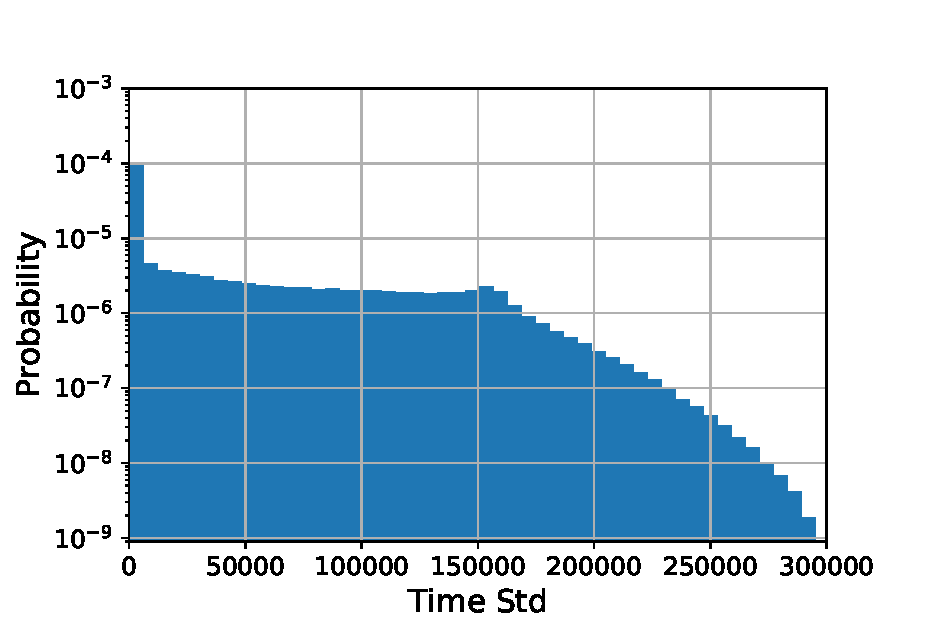
\includegraphics[width=0.22\textwidth]{fig/all_time_std_pdf.eps}
    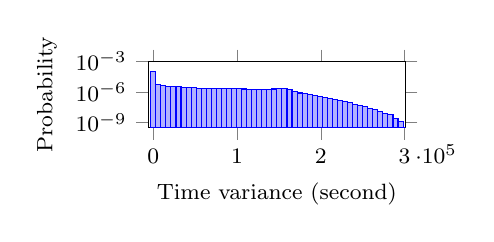
\begin{tikzpicture}
\begin{axis}[ymax=0.001,ybar,ymode=log,bar width=6023.807139652907,log origin=infty,xmin=-6023.807139652907,ytick align=outside,enlargelimits=0,
width=.40\textwidth,
height=.20\textwidth,
ylabel=Probability,
xlabel=Time variance (second),
every x tick scale label/.style={at={(xticklabel cs:1)},anchor=south west},
  label style={font=\footnotesize},
tick label style={font=\footnotesize} ,
]
\addplot  plot coordinates {
(0.0, 9.451382865223466e-05)
(6023.807139652907, 5.4237855234498505e-06)
(12047.614279305813, 4.160561994558263e-06)
(18071.421418958722, 3.567714777734051e-06)
(24095.228558611627, 3.385128656276782e-06)
(30119.03569826453, 3.165308635083816e-06)
(36142.842837917444, 2.9615307529739165e-06)
(42166.64997757035, 2.6626153921894407e-06)
(48190.45711722325, 2.5490152149843527e-06)
(54214.26425687616, 2.3890921746281617e-06)
(60238.07139652906, 2.275444535473124e-06)
(66261.87853618198, 2.248248838151831e-06)
(72285.68567583489, 2.156718467673447e-06)
(78309.49281548779, 2.138350693042835e-06)
(84333.2999551407, 2.0591366985764506e-06)
(90357.1070947936, 2.0862137410228693e-06)
(96380.9142344465, 2.0135969575995206e-06)
(102404.72137409942, 2.000948347937872e-06)
(108428.52851375232, 1.9544830989369192e-06)
(114452.33565340523, 1.9188391745245435e-06)
(120476.14279305813, 1.8834088288869425e-06)
(126499.94993271104, 1.8642104701322076e-06)
(132523.75707236395, 1.8633324240581345e-06)
(138547.56421201685, 1.8347365992133192e-06)
(144571.37135166978, 1.9392715439779758e-06)
(150595.17849132267, 2.1352419353211166e-06)
(156618.98563097557, 2.1487685910568386e-06)
(162642.79277062847, 1.6649889352174985e-06)
(168666.5999102814, 1.0367825656806102e-06)
(174690.4070499343, 7.939434987619423e-07)
(180714.2141895872, 6.496829018892185e-07)
(186738.02132924012, 5.151757357311993e-07)
(192761.828468893, 4.3131047016972446e-07)
(198785.6356085459, 3.5105231280444205e-07)
(204809.44274819884, 2.852225882239295e-07)
(210833.24988785174, 2.272003544101756e-07)
(216857.05702750463, 1.7961974958539996e-07)
(222880.86416715756, 1.4827113164349042e-07)
(228904.67130681046, 1.1445449230418602e-07)
(234928.47844646336, 8.545524088479658e-08)
(240952.28558611625, 6.371766780774196e-08)
(246976.09272576918, 4.777045262457526e-08)
(252999.89986542208, 3.780344313509607e-08)
(259023.70700507498, 2.6009148572545693e-08)
(265047.5141447279, 1.8557622430411254e-08)
(271071.3212843808, 1.31232291611476e-08)
(277095.1284240337, 8.305841241232658e-09)
(283118.9355636866, 5.624241069063257e-09)
(289142.74270333955, 2.7053311471443514e-09)
(295166.54984299245, 1.3526655735721757e-09)
(301190.35698264535, 3.0850267467435584e-10)
};\end{axis}
\end{tikzpicture}

	%\caption{Example of a high-order proximity caption.}
	}&
	\subfigure[Histogram of time std for hack\&phish nodes.]{
		\label{fig:asymmetric}
		%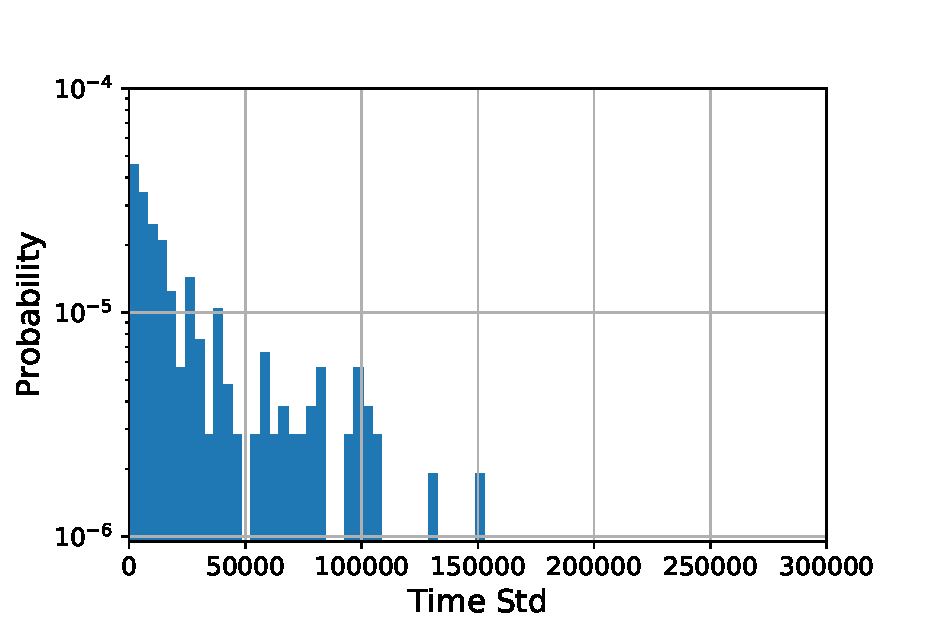
\includegraphics[width=0.22\textwidth]{fig/fake_time_std_pdf.eps}
    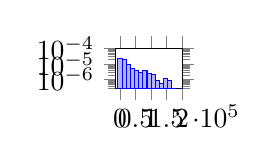
\begin{tikzpicture}
\begin{axis}[ymax=0.0001,ybar,ymode=log,bar width=13410.783587930588,log origin=infty,xmin=-13410.783587930588,ytick align=outside,enlargelimits=0,
width=.20\textwidth,
every x tick scale label/.style={at={(xticklabel cs:1)},anchor=south west},
]
\addplot  plot coordinates {
(0.0, 2.1630081044550223e-05)
(13410.783587930588, 1.9637836737815332e-05)
(26821.567175861175, 8.822796215540222e-06)
(40232.350763791765, 5.122913931604e-06)
(53643.13435172235, 3.699882283936222e-06)
(67053.91793965294, 2.8460632953355556e-06)
(80464.70152758353, 3.984488613469778e-06)
(93875.48511551411, 2.561456965802e-06)
(107286.2687034447, 2.2768506362684445e-06)
(120697.0522913753, 8.538189886006666e-07)
(134107.83587930587, 5.692126590671111e-07)
(147518.61946723645, 1.1384253181342222e-06)
(160929.40305516706, 8.538189886006666e-07)
(174340.18664309764, 2.8460632953355556e-07)
(187750.97023102822, 0.0)
(201161.75381895882, 2.8460632953355556e-07)
};\end{axis}
\end{tikzpicture}

	}
\end{tabular}
\caption{Examples.}
\end{figure}

Specially, we extend the pre-processing scheme to adapt our model. First we construct four relation graphs, which contains ETH transfer graph, contract creation graph, contract invocation graph and mining reward graph. In each graph, repeated edges between the same node pair are merged via the method introduced in section \ref{section:time}.

Last, a test set of accounts with label introduced before is provided to evaluate classification accuracy. It is hard to reveal the identity of addresses since the anonymity of blockchain. We obtain these labeled examples in two ways, \emph{Etherscan}\footnote{Etherscan LabelCloud, https://etherscan.io/labelcloud} and \emph{Searchain}\footnote{Searchain, http://www.searchain.io/}.




\subsection{Experimental Set-Up and Baselines}
Unless otherwise noted,

As a baseline for our experiments, we compare against state-of-the-art classification accuracy from \textcolor{red}{XXX, XXX, XXX and XXX}.
\begin{table*}
\footnotesize
\centering
\caption{}
\resizebox{\textwidth}{17mm}{
\begin{tabular}{l|ccc|ccc|ccc|ccc|ccc}
\toprule
& \multicolumn{3}{c|}{Deepwalk} & \multicolumn{3}{c|}{GCN} & \multicolumn{3}{c|}{rGCN} & \multicolumn{3}{c|}{rGCN+asymmetric proximity} & \multicolumn{3}{c|}{Ours} \\
\midrule
& \textbf{Precision} & \textbf{Recall} & $\mathbf{F_1}$ & \textbf{Precision} & \textbf{Recall} & $\mathbf{F_1}$ & \textbf{Precision} & \textbf{Recall} & $\mathbf{F_1}$ & \textbf{Precision} & \textbf{Recall} & $\mathbf{F_1}$ & \textbf{Precision} & \textbf{Recall} & $\mathbf{F_1}$ \\
\midrule
 phish and hack & & & &0.614 & 0.273 & 0.378 & 0.700& 0.778& 0.737& 0.720& 0.727& 0.724& 0.714& 0.758& 0.735\\
 token contract & & & &0.634& 0.459& 0.533& 0.930& 0.949& 0.939& 0.958& 0.939& 0.949& 0.958& 0.939& 0.949\\
 exchange deposit & & & &0.526& 0.400& 0.455& 0.500& 0.280& 0.359& 0.615& 0.640& 0.628& 0.556& 0.600& 0.579\\
 exchange root & & & &0.579& 0.743& 0.650& 0.913& 0.600& 0.724& 0.862& 0.714& 0.781& 0.828& 0.686& 0.750\\
 pool & & & &0.344& 0.500& 0.407& 1.000& 0.636& 0.778& 0.842& 0.727& 0.781& 1.000& 0.727& 0.842\\
 miner & & & &0.696& 0.390& 0.500& 0.905& 0.927& 0.916& 0.826& 0.927& 0.874& 0.841& 0.902& 0.871\\
 primary market & & & & 0.238& 0.161& 0.192& 0.786& 0.355& 0.489& 0.680& 0.548& 0.607& 0.750& 0.484& 0.588\\
 ICO wallet & & & & 0.539& 0.184& 0.275& 0.677& 0.552& 0.609& 0.769& 0.526& 0.625& 0.742& 0.605& 0.668\\
 \midrule
 average & & & & 0.566& 0.378& 0.436& 0.807& 0.725& 0.751& 0.806& 0.761& 0.779& \bf{0.811}& \bf{0.764}& \bf{0.782}\\
\bottomrule
\end{tabular}
}
\end{table*}

% \begin{table}
% \centering
% \caption{}
% \begin{tabular}{l|ccc}
% \toprule
% \textbf{Model} & \textbf{Precision}  & \textbf{Recall} & $\mathbf{F_1}$  \\
% \midrule
%  Deepwalk & & & \\
%  GCN & & & \\
%  rGCN & & & \\
%  Our & & & \\
% \midrule
%  w/o time-density& & & \\
%  w/o asymmetric proximity & & & \\
% \bottomrule
% \end{tabular}
% \end{table}

All embedding and classification programs were run on the server, which includes Intel Xeon E5 CPU with 55 processors and 128GB of memory, and the GPU used for deep learning is Nvidia 1080Ti.

\subsection{Results}


%These data are collected

%%% Local Variables:
%%% mode: latex
%%% TeX-master: "analysis"
%%% End:

\input{relatedworks.tex}
% !TEX root = main.tex

\section{Conclusion}
\label{sec:conclusion}
In this paper, we have studied the deanonymization in Ethereum and similar DApp platform blockchains. An approach called I$^2$GL has been proposed to infer user identity using graph deep learning. Since the blockchain transaction graph is too large to be handled by traditional graph analytics methods, we use graph embedding technique to convert the original graph into a low-dimensional one. Furthermore, we exploit unique features of blockchain transaction graphs, such as time-density, second-order proximity, and asymmetric proximity, and correspondingly propose a series of enhancement. We evaluate I$^2$GL by comparing it with three state-of-the-art and experimental results on Ethereum transaction records show the superiority of I$^2$GL.

\bibliography{reference}

\end{document}

%%% Local Variables:
%%% mode: latex
%%% TeX-master: t
%%% End:
